% vim: spell spelllang=en:
%! TEX root = **/main.tex
\documentclass[12pt, oneside]{article}
\usepackage[a4paper, left=2.5cm, right=2.5cm, top=2.5cm, bottom=2.5cm]{geometry}

\usepackage[T1]{fontenc}
\usepackage[utf8]{inputenc} % Use unicode for input
%\usepackage{lmodern}

\usepackage[english]{babel}

%% Bibliography:
%\usepackage{comment}
%\usepackage[
    %backend=biber,
    %style=numeric,
%]{biblatex}
%\DeclareNameAlias{default}{last-first}

%\usepackage{csquotes}       % For bibliography quotations
%\DeclareQuoteAlias{spanish}{catalan}

%\addbibresource{biblio.bib}
%% see:
%% https://www.sharelatex.com/learn/Bibliography_management_in_LaTeX#The_bibliography_file

%\usepackage{datetime} % Customize date
%% \monthyeardate\today gives the date without the day
%\newdateformat{monthyeardate}{%
    %\monthname[\THEMONTH], \THEYEAR}

% For cross references
\usepackage{xcolor}
\usepackage{color}
\usepackage[colorlinks = true]{hyperref}
\usepackage[english]{varioref}
%\usepackage{cleveref}
%hyperref configuration so that it doesn't contrast so much colorlinks,
\hypersetup{
   linkcolor={black},
   citecolor={black},
   %linkcolor={red!50!black},
   %citecolor={blue!50!black},
   urlcolor={blue!80!black}
}

\usepackage{mathtools}  % amsmath + more
\usepackage{amsthm}     % Theorem enviroment
\usepackage{amssymb}    % More symbols
\usepackage{amstext}    % Text inside mathenv

\usepackage{relsize}    % Bigger math with mathlarger{___}
\usepackage{nicefrac}   % nice fractions in one line

\usepackage[export]{adjustbox}  % Adjust table size
\usepackage{float}              % Force tables and images position (H and H!)
\usepackage{wrapfig}            % Wrap images like in HTML

%\usepackage{tabularx, colortbl, booktabs}    % Better tables
%\usepackage{tabularx, colortbl, booktabs}    % Better tables
%\usepackage{longtable}                      % Multiple page table
\usepackage{xltabular}
\usepackage{colortbl, booktabs}    % Better tables

% bug booktabs + xltabular
\makeatletter
\def\@BTrule[#1]{%
  \ifx\longtable\undefined
    \let\@BTswitch\@BTnormal
  \else\ifx\hline\LT@hline
    \nobreak
    \let\@BTswitch\@BLTrule
  \else
     \let\@BTswitch\@BTnormal
  \fi\fi
  \global\@thisrulewidth=#1\relax
  \ifnum\@thisruleclass=\tw@\vskip\@aboverulesep\else
  \ifnum\@lastruleclass=\z@\vskip\@aboverulesep\else
  \ifnum\@lastruleclass=\@ne\vskip\doublerulesep\fi\fi\fi
  \@BTswitch}
\makeatother

% Split cell in lines and more formating options inside table
\usepackage{array, multirow, multicol, makecell}

%\usepackage{subcaption}                     % Subfigures
%\usepackage[framemethod=tikz]{mdframed}     % Custom frames

%\usepackage[bottom]{footmisc} % Footnotes at bottom of page

%\usepackage[alsoload=hep]{siunitx}          % SI units and uncertainties
%\sisetup{locale = FR}                       % Commas and so on for spanish
%\sisetup{separate-uncertainty=true}
%\sisetup{
  %per-mode=fraction,
  %fraction-function=\nicefrac
%}

%\usepackage{tikz}
%%\usetikzlibrary{arrows}
%%\usetikzlibrary{scopes}
%\usetikzlibrary{babel}

%\usepackage{listings}       % For code blocks

%% Custom code highlight
%\definecolor{codegreen}{rgb}{0,0.6,0}
%\definecolor{codegray}{rgb}{0.5,0.5,0.5}
%\definecolor{codepurple}{rgb}{0.58,0,0.82}
%\definecolor{backcolour}{rgb}{0.95,0.95,0.92}
%\definecolor{lightblue}{RGB}{135,206,250}

%\lstdefinestyle{mystyle}{ backgroundcolor=\color{backcolour},
    %commentstyle=\color{codegreen}, keywordstyle=\color{blue},
    %numberstyle=\tiny\color{codegray}, stringstyle=\color{red},
    %identifierstyle=\color{black}, basicstyle=\footnotesize,
    %%breakatwhitespace=false,
    %breaklines=true,
    %%captionpos=b,                    keepspaces=true,
    %numbers=left,                    numbersep=5pt,
    %showspaces=false,
    %%showstringspaces=false, showtabs=false,
    %tabsize=4
%}
%\lstset{style=mystyle}

\newcommand{\whitepage}{
    \clearpage\thispagestyle{empty}\addtocounter{page}{-1} \newpage \clearpage
}

% Add command before appendix session for page numbering: A-1
%\newcommand{\appendixpagenumbering}{
    %\break
    %\pagenumbering{arabic}
    %\renewcommand{\thepage}{\thesection-\arabic{page}}
%}

%% Custom Math operators (functions not in italic in math mode):
%\DeclareMathOperator{\arcsec}{arcsec}
%\DeclareMathOperator{\arccot}{arccot}
%\DeclareMathOperator{\arccsc}{arccsc}
%\DeclareMathOperator{\cis}{cis}

\usepackage{pdflscape}
\usepackage{pifont}

\usepackage{pdfpages}
\usepackage{comment}
\usepackage{xspace}


\title{MD - \airbnb Barcelona Listings}
\author{
    Aleix Bon\'e\\
    Eduard Bosch\\
    David Gili\\
    Albert Mercad\'e
}
\date{\today}

\setbeamercolor{background canvas}{bg=white}

\graphicspath{{../../analysis/plots/}{images}}

\newcommand{\airbnb}{\emph{Airbnb}\xspace}
\newcommand{\NA}{\emph{NA}\xspace}

\newcommand{\profiling}[3]{
\begin{figure}[H]
    \centering
    \includegraphics[width=0.8\textwidth]{prof-c3-#1-#2}
    \caption{#3}%
    \label{fig:prof-#1-#2}
\end{figure}
}

\newcommand{\fig}[3][0.6]{
    \begin{figure}[H]
        \centering
        \includegraphics[width=#1\linewidth]{#2}
        \caption{#3}%
        \label{fig:#2}
    \end{figure}
}

\newcommand{\hibp}[2]{
    \begin{figure}[H]
        \centering
        \includegraphics[width=0.6\linewidth]{desc-#1-hi_bp}
        \caption{Histogram \& Boxplot of #2}%
        \label{fig:#1}
    \end{figure}
}

\newcommand{\tabn}[2]{
    \begin{table}[H]
        \centering
        \caption{Extended summary statistics of #2}%
        \label{tab:#1}
        \input{../../analysis/tables/desc-#1-ext_sum}
    \end{table}
}

\newcommand{\factorialmap}[2]{
    \begin{figure}[H]
        \centering
        \includegraphics[width=0.7\linewidth]{pca_fact-plane_#1_#2-bi}
        \caption{PCA plane #1 vs #2}%
        \label{fig:plane_#1-#2}
    \end{figure}
}

\newcommand{\fign}[2]{
    %\sssfig{#2}
    \hibp{#1}{#2}
    %\tabn{#1}{#2}
}

\newcommand{\figf}[2]{
%\sssfig{#2}
\begin{figure}[H]
    \begin{minipage}{0.39\linewidth}
            \centering
            \includegraphics[width=\linewidth]{desc-#1-bar}
    \end{minipage}
    \begin{minipage}{0.39\linewidth}
            \centering
            \includegraphics[width=\linewidth]{desc-#1-pie}
    \end{minipage}
    \caption{Barplot \& Pie chart of #2}%
    \label{fig:#1}
\end{figure}


%\begin{table}[H]
%    \centering
%    \caption{Table of #2 frequency}%
%    \label{tab:#1}
%    \input{../../analysis/tables/desc-#1-freq}
%\end{table}
}

%\hfuzz=3pt
%\vfuzz=3pt

%1. Slide with title, name of all group components, delivery date
%2. Slide with outline of talk
%3. Slide with topics addressed, goals of the work and urls from data sources, overview of BD structure and variables analyzed
%4. Slide with the Data mining process schema
%5. Slide with the descriptive analysis of one numerical variable and one qualitative variable
%6. Slide synthesizing univariate descriptive analysis
%7. Slide with additional descriptive analysis issues when relevant
%8. Slide describing preprocessing steps (if required add additional slides for any specific aspect to be commented)
%9. Slide with PCA specificacions, screeplot
%10. Slide wtith first factorial plane for PCA (eventually additional slides for othe planes retained). Lack of visibility of map
%penalizes.
%11. Slide with conlusions of PCA
%12. Slide describing the clustering process followed and resulting dendrogramm
%13. Slide describing which tools of class interpretation you have been used
%14. Slide with CPG or eventual profiling graphs or numerical information about clusters to be highlighted (whenever possible,
%synthesize important graphics in a single slide... evenctually you can add some extra slide)
%15. Slide with final class profiling (synthesis with description of class characteristics)
%16. Slide with comparison of conclusions between PCA and clustering
%17. Slide with conclusions
%18. Slide with original and final scheduling

\begin{document}

\maketitle

\section{Outline}
\begin{frame}{Outline}
\begin{scriptsize}
    \tableofcontents
\end{scriptsize}
\end{frame}

%3. Slide with topics addressed, goals of the work and urls from data sources, overview of BD structure and variables analyzed
\section{Data source}
\begin{frame}{Our Dataset}
\begin{center}
    Inside Airbnb Barcelona Listings - 24/08/2020\footnote[frame]{Dataset URL: \url{http://data.insideairbnb.com/spain/catalonia/barcelona/2020-08-24/data/listings.csv.gz}}

\vspace{5 mm}

\begin{columns}[t]
    \column{0.3\textwidth}
    20,703 data records
    
    9.01\% of missing data
    
    74 variables
    \small
    \begin{itemize}[topsep=0pt]
        \itemsep-0.25em
    	\item[--] 30 categorical
    	\item[--] 38 numerical
    	\item[--] 6 boolean
    \end{itemize}
    \normalsize
    
    \column{0.3\textwidth}
    Host information
    \small
    \begin{itemize}[topsep=0pt]
        \itemsep-0.5em
    	\item[--] Acceptance rate
    	\item[--] Listings count
    	\item[--] \dots
    \end{itemize}
    \normalsize
    Listing information
    \small
    \begin{itemize}[topsep=0pt]
        \itemsep-0.5em
    	\item[--] Price
    	\item[--] Reviews
    	\item[--] \dots
    \end{itemize}
    \normalsize
\end{columns}

\end{center}
\end{frame}


\begin{frame}{Goals}
\begin{quote}
The focus of the project will be to analyse whether or not factors
such as price, availability or neighbourhood impact whether or not the final
user review is positive or negative.
\end{quote}
\end{frame}

%4. Slide with the Data mining process schema
\section{Data mining process scheme}
\begin{frame}{Data mining process}
\begin{figure}[H]
    \centering
    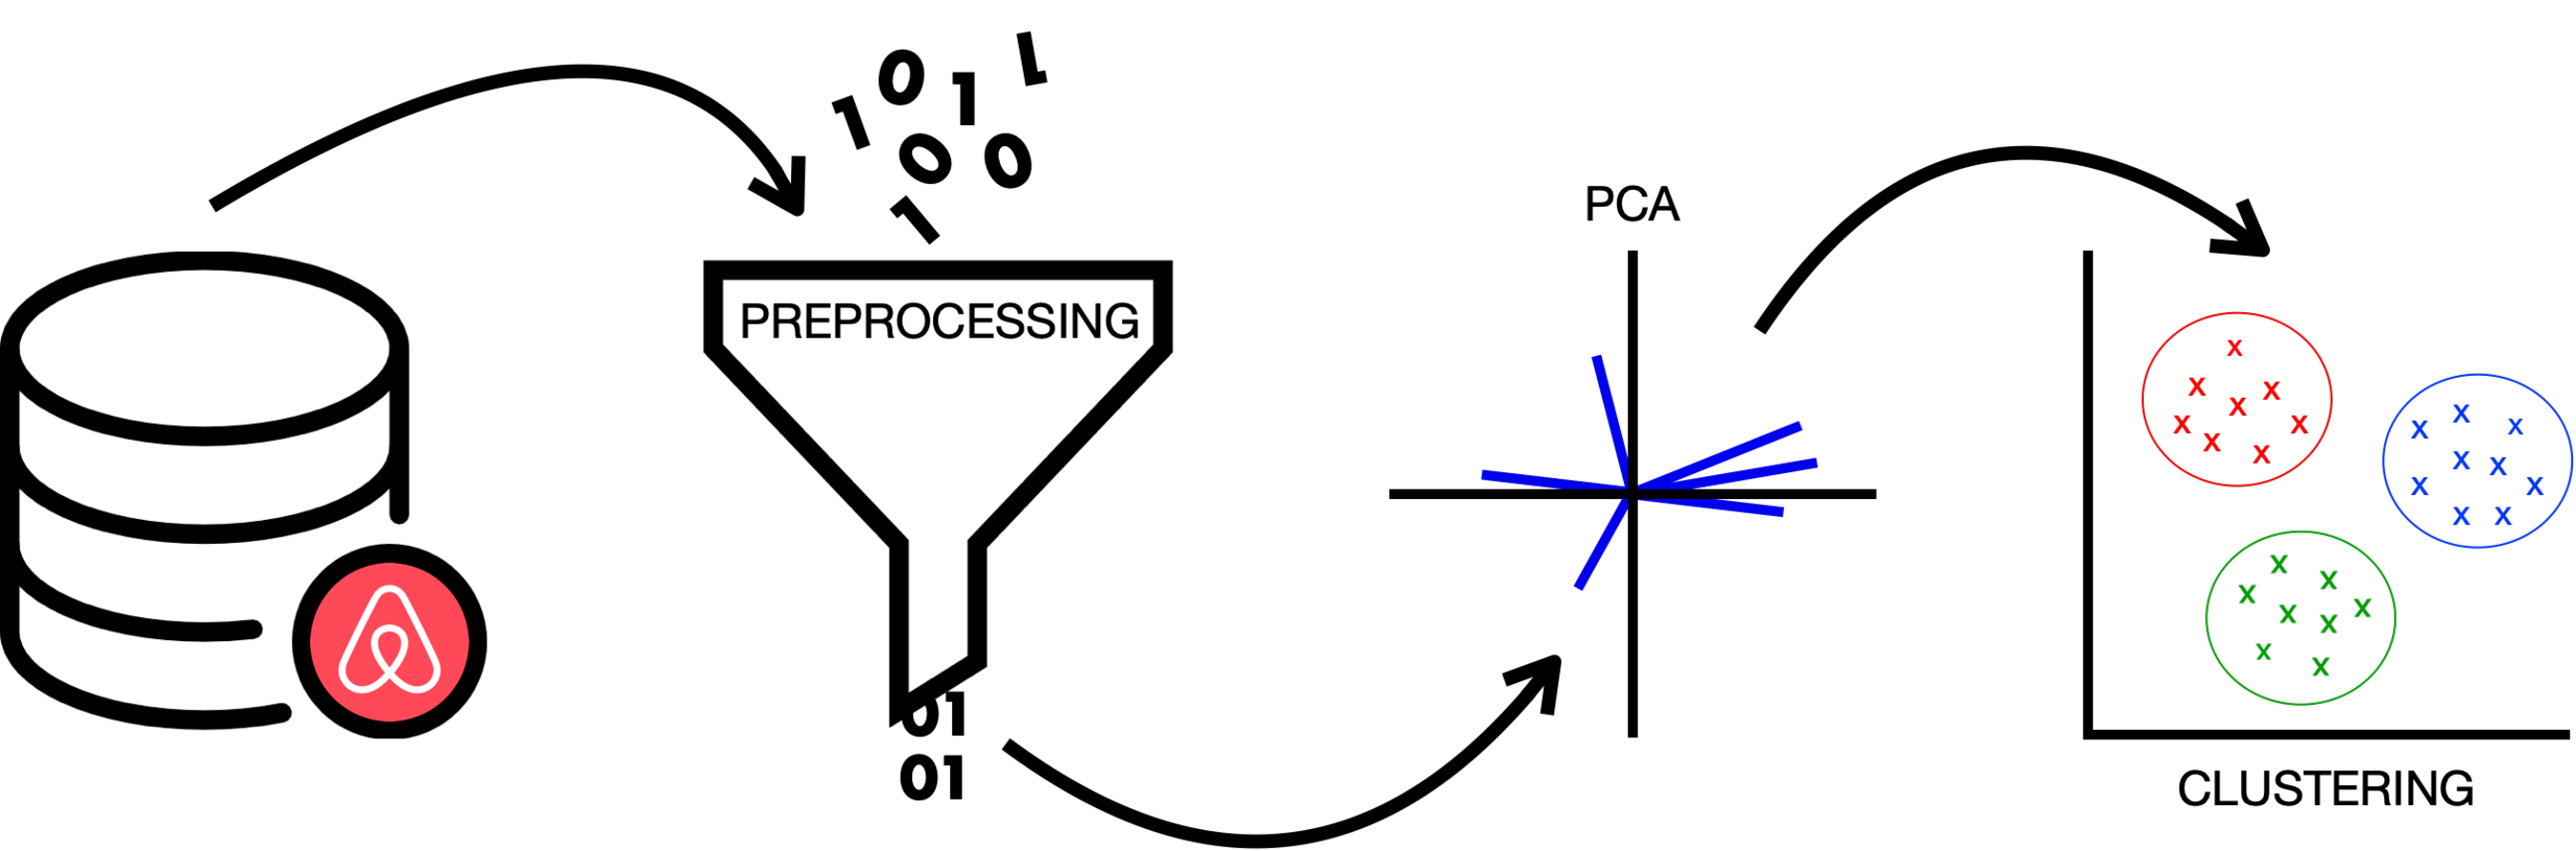
\includegraphics[width=0.75\linewidth]{../final/images/workflow}
    %\caption*{Our data mining workflow}
\end{figure}
\end{frame}

%5. Slide with the descriptive analysis of one numerical variable and one qualitative variable
\section{Descriptive analysis}
\begin{frame}{Numerical variable}
\vspace{0.7em}
\fign{review_scores_rating}{review scores rating}
\end{frame}

\begin{frame}{Qualitative variable}
\vspace{1.5em}
\figf{neighbourhood_group_cleansed}{neighbourhood group cleansed}
\end{frame}


%6. Slide synthesizing univariate descriptive analysis
\section{Univariate descriptive analysis}
\begin{frame}{Univariate descriptive analysis}
\end{frame}

\section{Bivariate descriptive analysis}
\begin{frame}{Bivariate descriptive analysis}
\fig{bivar-reviews_per_month-review_scores_rating}{Score rating vs reviews per month}
\end{frame}

%7. Slide with additional descriptive analysis issues when relevant
\begin{frame}{Issues}
\fign{host_listings_count}{Host listings count}
\end{frame}

%8. Slide describing preprocessing steps (if required add additional slides for any specific aspect to be commented)
\section{Preprocessing}
\begin{frame}{Preprocessing steps}
\large
\begin{itemize}
     \itemsep0.5em
     \item Determining working matrix
     \item Missing 
     \begin{itemize}
         \itemsep0.25em
         \item Numerical $\rightarrow$ Knn Algorithm
         \item Categorical $\rightarrow$ New 'Unknown' category 
     \end{itemize}
     \item Outliers
     \item Errors
     \item Derivation of new categorical variables
\end{itemize}
\normalsize
\end{frame}

%9. Slide with PCA specificacions, screeplot
\section{PCA}
\begin{frame}{Screeplot}
\begin{figure}[H]
    \centering
    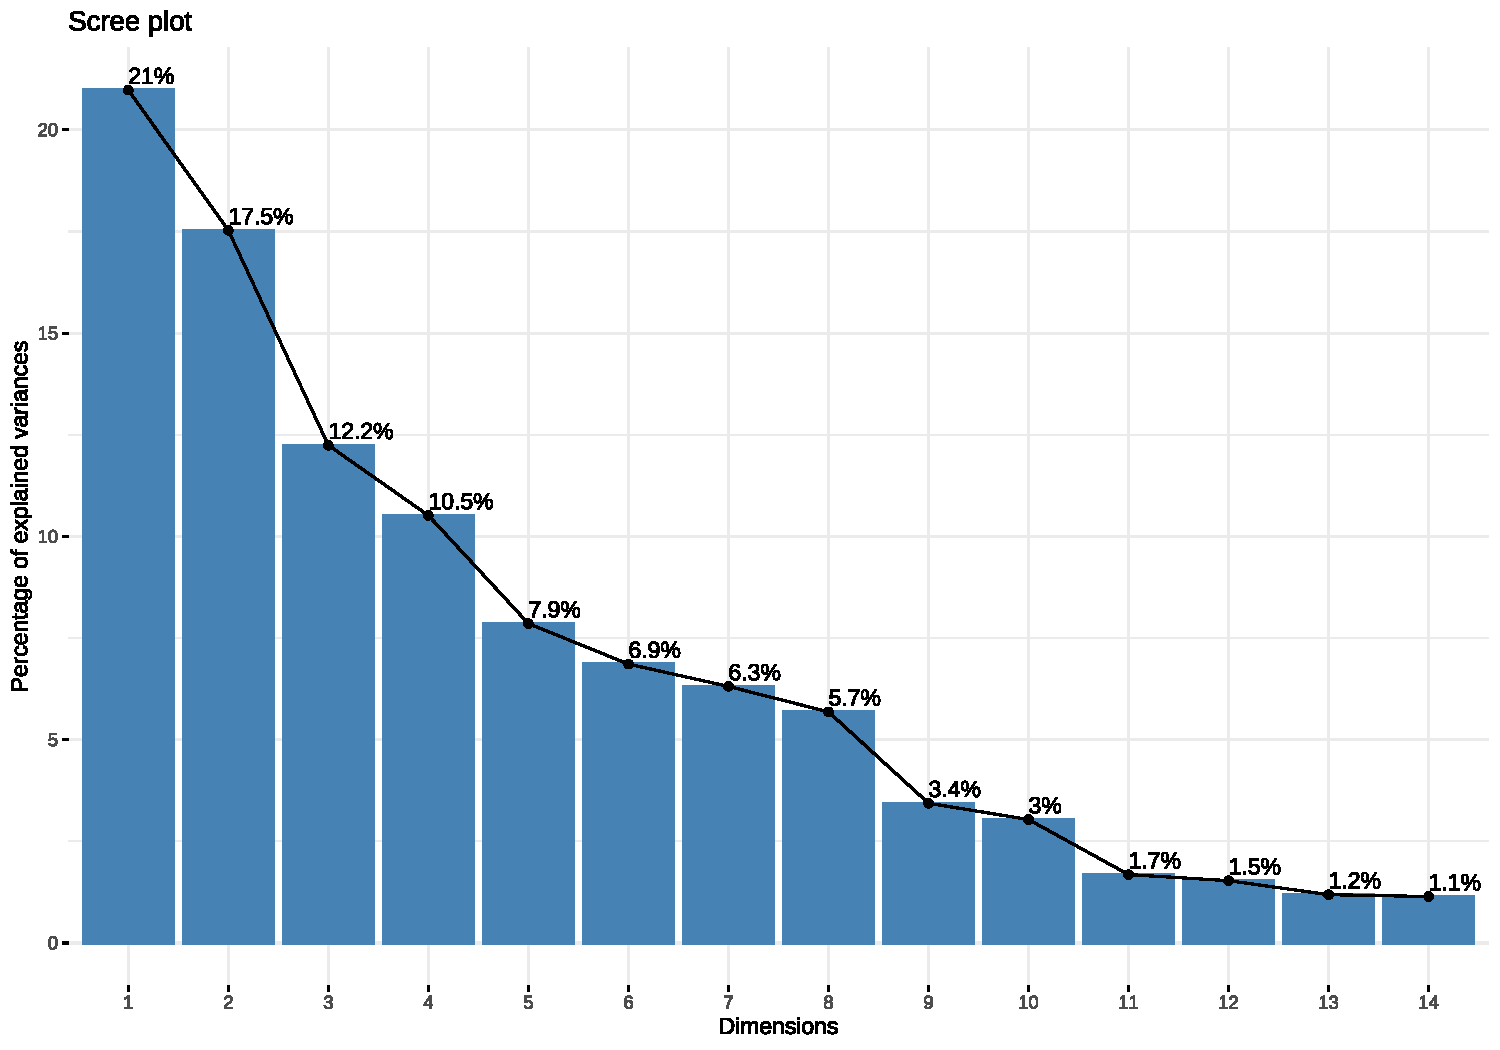
\includegraphics[width=0.7\linewidth]{pca_fact-screeplot} % PCA-inertia_cum
    \caption{PCA inertia}%
    \label{fig:pca_inertia}
\end{figure}
\end{frame}

%10. Slide wtith first factorial plane for PCA (eventually additional slides for othe planes retained). Lack of visibility of map
%penalizes.
\begin{frame}{First factorial plane}
\factorialmap{1}{2}
\end{frame}

\begin{frame}{factorial plane 1 v 3} %  o lo k sigui
\factorialmap{1}{3}
\end{frame}

\begin{frame}{factorial plane 2 v 4} %  o lo k sigui
\factorialmap{2}{4}
\end{frame}

%11. Slide with conlusions of PCA
\begin{frame}{Conclusions}
Variables that contribute the most to each factorial axis:
\begin{itemize}
     \item Axis 1: accommodates, beds and bedrooms (direct relation)
     \item Axis 2: review scores ratings (direct relation)
     \item Axis 3: number of reviews (direct relation)
     \item Axis 4: availability (direct relation)
\end{itemize}
\end{frame}

%12. Slide describing the clustering process followed and resulting dendrogramm
\section{Clustering}
\begin{frame}{Process}
    \begin{figure}[H]
    \centering
    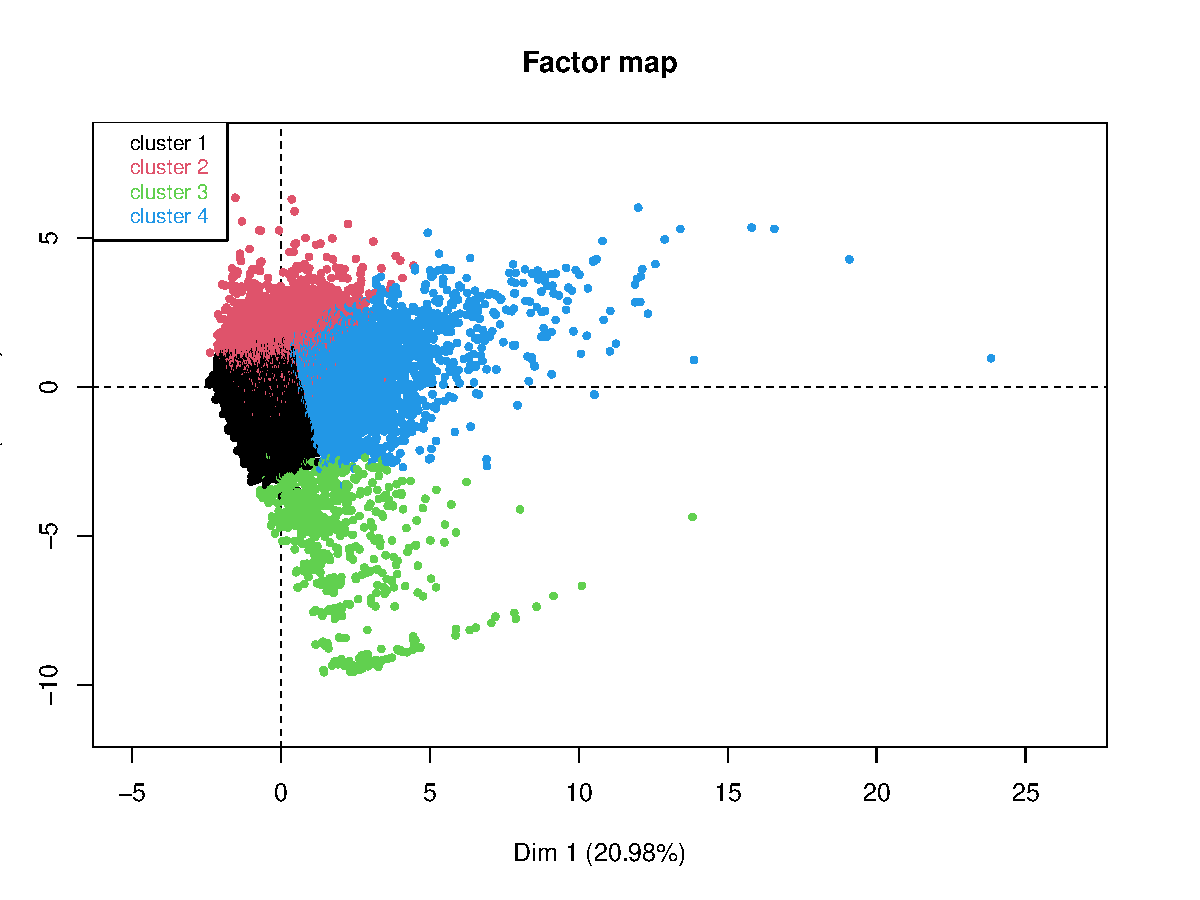
\includegraphics[width=0.7\linewidth]{factor_map}
    \caption{Clusters on PCA}%
    \label{fig:clusters-pca}
    \end{figure}
\end{frame}

\begin{frame}{Resulting Dendogram}
\begin{figure}[H]
    \centering
    %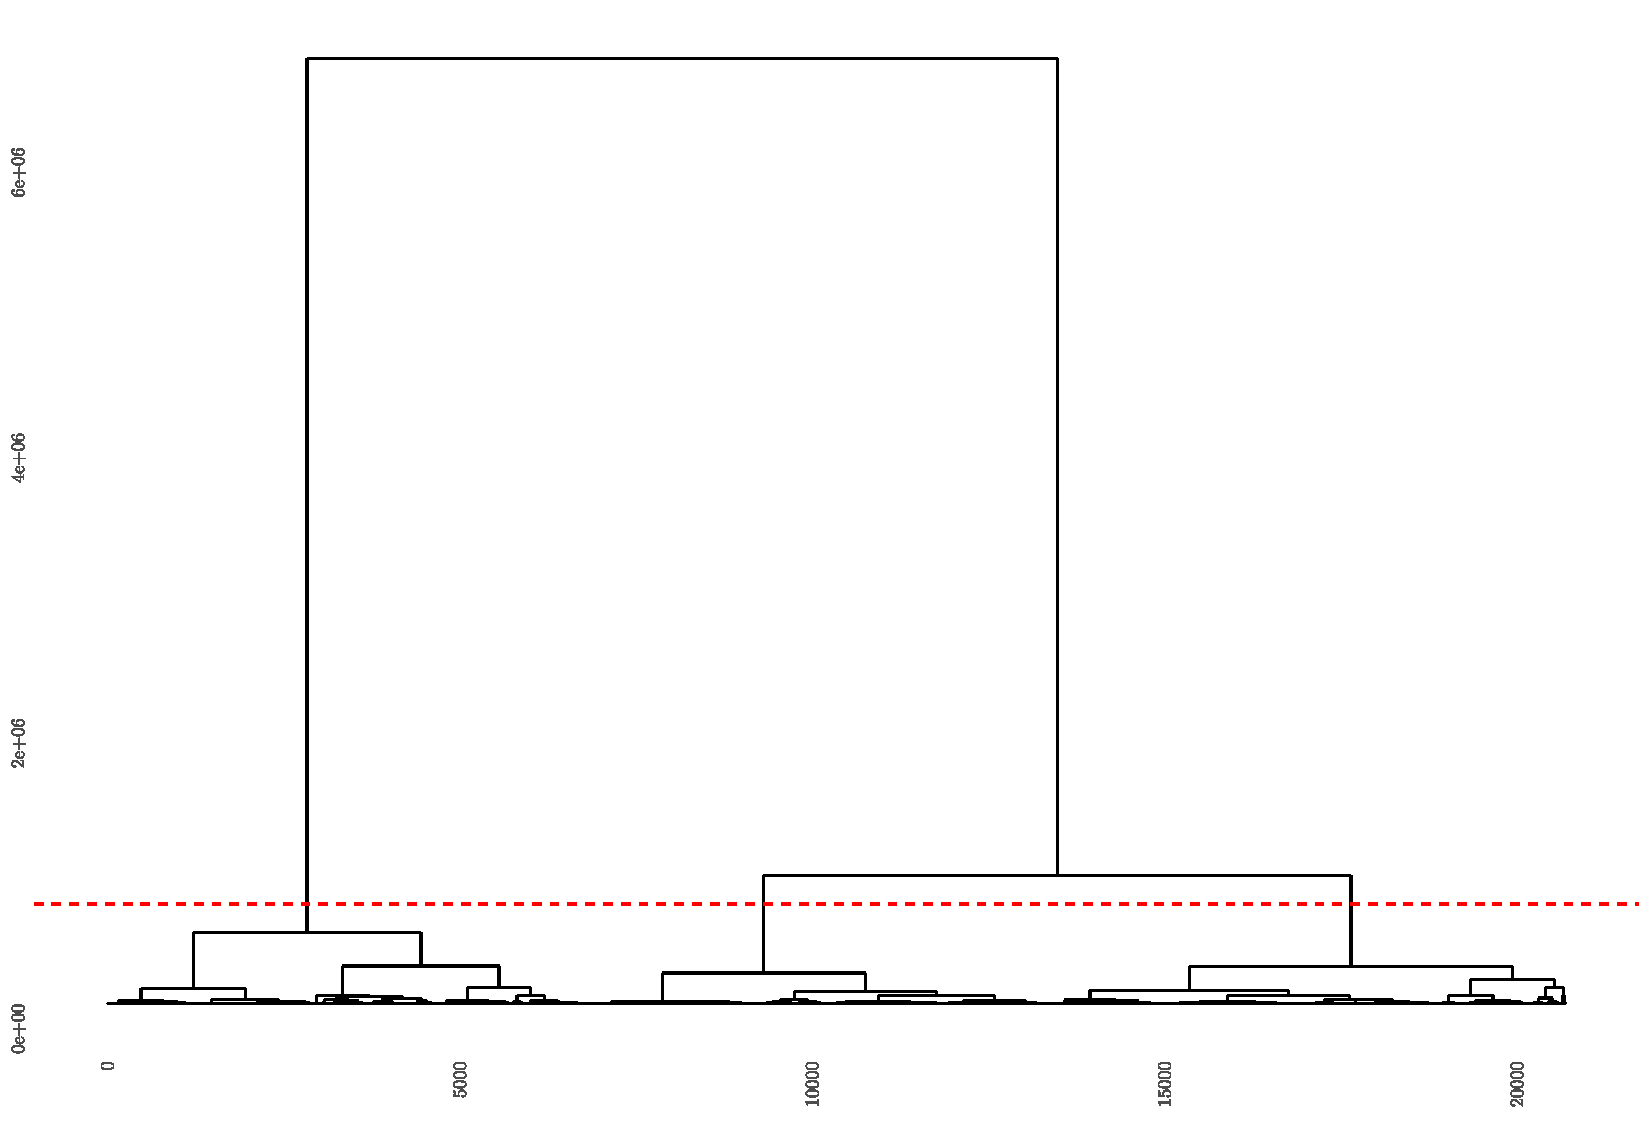
\includegraphics[width=0.8\linewidth]{dendo}
    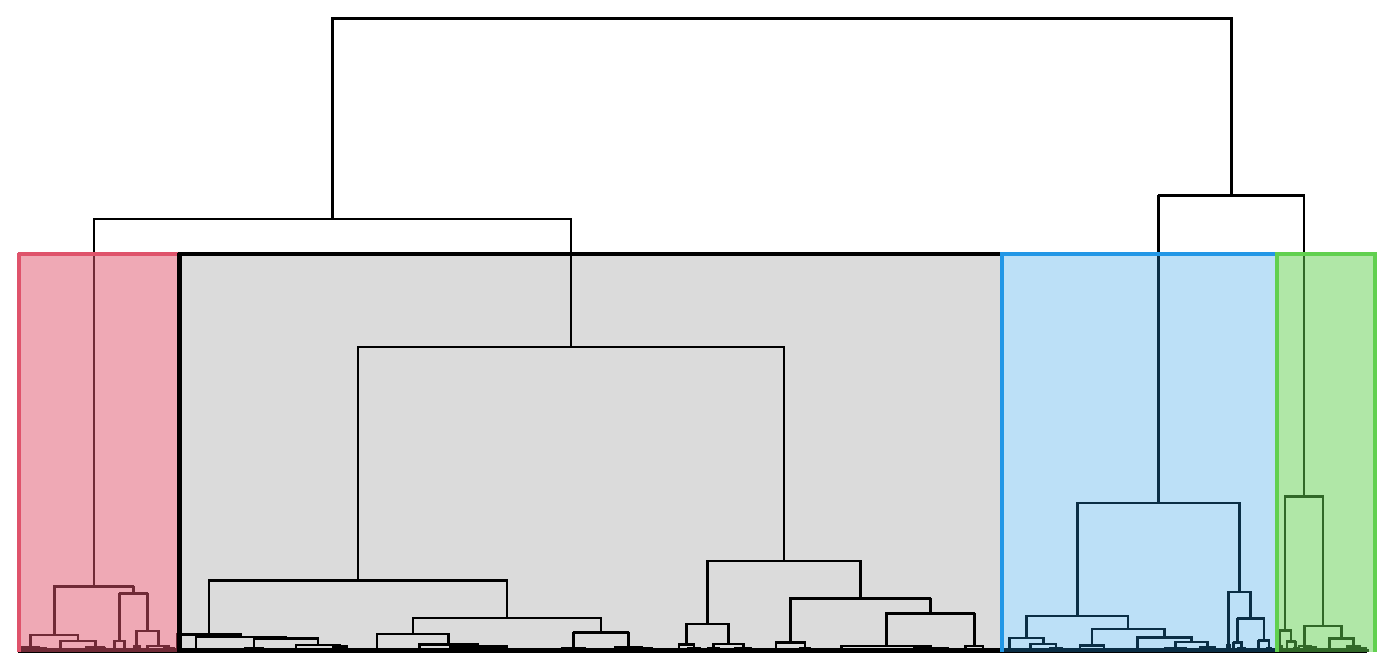
\includegraphics[width=0.8\linewidth]{cluster-dendo-h3-color}
    %\caption{Cluster Dendogram}%
    \label{fig:dendogram-final}
\end{figure}
\end{frame}


%13. Slide describing which tools of class interpretation you have been used
\begin{frame}{Class interpretation Dendogram}
\end{frame}

%14. Slide with CPG or eventual profiling graphs or numerical information about clusters to be highlighted (whenever possible,
%synthesize important graphics in a single slide... evenctually you can add some extra slide)
\section{Profiling}
\begin{frame}[allowframebreaks]{Profiling}

\begin{columns}
\begin{column}{0.5\textwidth}
\profiling{review_scores_rating}{vi}{Review scores rating}
\end{column}
\begin{column}{0.5\textwidth}  %%<--- here
\profiling{reviews_per_month}{bp}{Reviews per month}
\end{column}
\end{columns}

\framebreak

\begin{columns}
\begin{column}{0.5\textwidth}
\profiling{accommodates}{bp}{Listing's allowance}
\end{column}
\begin{column}{0.5\textwidth}  %%<--- here
\profiling{bedrooms}{meanp}{Median number of bedrooms}
\end{column}
\end{columns}
\end{frame}

%15. Slide with final class profiling (synthesis with description of class characteristics)
\begin{frame}{Final class profiling}
\begin{figure}[H]
\centering
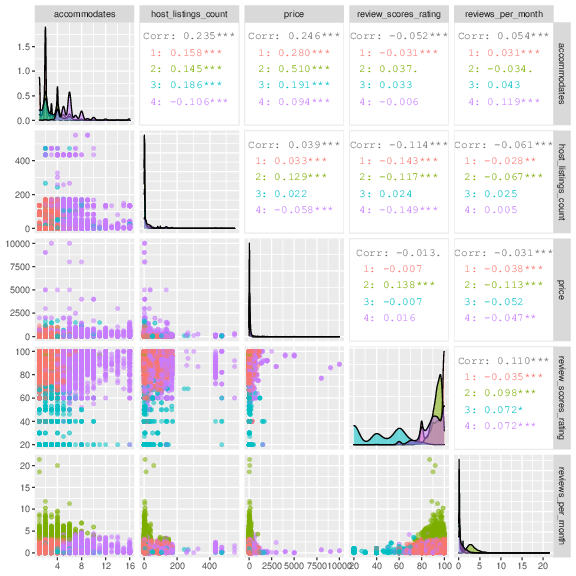
\includegraphics[height=0.9\textheight]{pairs.png}
\end{figure}
\end{frame}
%16. Slide with comparison of conclusions between PCA and clustering


%17. Slide with conclusions
\section{Conclusions}
%\begin{frame}{Conclusions}
%\end{frame}

%18. Slide with original and final scheduling
\section{Working plan}
\begin{frame}{Original scheduling}
\centering
\vspace{1.4em}
\scalebox{0.25}{%\begin{minipage}{1.20\textwidth}
% vim: spell spelllang=en:
%! TEX root = **/00-main.tex

\begin{ganttchart}[
vgrid={*{6}{draw=none}, dotted},
x unit=.75cm,
y unit title=1cm,
y unit chart=1cm,
    time slot format=isodate
    %]{2020-09-15}{2020-10-07}
    ]{2020-09-15}{2020-10-28}
\gantttitlecalendar{month=name, day}
\ganttnewline

\ganttgroup{Motivation and Description}{2020-09-16}{2020-09-23}
\ganttnewline

\ganttgroup{Data source presentation}{2020-09-16}{2020-09-23}
\ganttnewline

\ganttbar{Description of data source}{2020-09-16}{2020-09-23}
\ganttnewline

\ganttgroup{Formal description of data structure}{2020-09-23}{2020-09-30}
\ganttnewline
\ganttbar{Metadata Table}{2020-09-23}{2020-09-25}
\ganttnewline
\ganttbar{Scope of study}{2020-09-25}{2020-09-30}
\ganttnewline

\ganttgroup{Description of preprocessing}{2020-09-23}{2020-09-27}
\ganttnewline

\ganttgroup{Basic statistical descriptive analysis}{2020-09-27}{2020-10-07}
\ganttnewline
\ganttbar{Univariate analysis}{2020-09-27}{2020-09-30}
\ganttnewline
\ganttbar{Bivariate analysis}{2020-10-01}{2020-10-04}
\ganttnewline
\ganttbar{Conclusion describing data}{2020-10-04}{2020-10-07}
\ganttnewline
%\end{ganttchart}
%
%\framebreak
%
%\begin{ganttchart}[
%vgrid={*{6}{draw=none}, dotted},
%x unit=.85cm,
%y unit title=1cm,
%y unit chart=1cm,
%    time slot format=isodate
%    ]{2020-10-07}{2020-10-28}
%\gantttitlecalendar{month=name, day}
%\ganttnewline

\ganttgroup{PCA analysis for numerical variables}{2020-10-07}{2020-10-14}
\ganttnewline
\ganttbar{Scree plot}{2020-10-07}{2020-10-11}
\ganttnewline
\ganttbar{Factorial map visualization}{2020-10-11}{2020-10-14}
\ganttnewline

\ganttgroup{Hierarchical Clustering}{2020-10-14}{2020-10-21}
\ganttnewline
\ganttbar{Clustering script}{2020-10-14}{2020-10-19}
\ganttnewline
\ganttbar{Description of data selected}{2020-10-19}{2020-10-21}
\ganttnewline
\ganttbar{Clustering method and metrics used}{2020-10-19}{2020-10-21}
\ganttnewline
\ganttbar{Resulting Dendogram}{2020-10-19}{2020-10-21}
\ganttnewline
\ganttbar{Discussion about number of clusters}{2020-10-19}{2020-10-21}
\ganttnewline
\ganttbar{Table with description of cluster size}{2020-10-19}{2020-10-21}
\ganttnewline

\ganttgroup{Profiling of clusters}{2020-10-21}{2020-10-28}
\ganttnewline
\ganttbar{Profiling graphs}{2020-10-21}{2020-10-28}
\ganttnewline

\end{ganttchart}

%\end{minipage}
}
\end{frame}

\begin{frame}{Final scheduling}
\centering
\vspace{1.4em}
\scalebox{0.25}{
% vim: spell spelllang=en:
%! TEX root = **/00-main.tex

\newgeometry{top=0.5cm, bottom=0.5cm, left=0.5cm, right=0.5cm}
\begin{landscape}

\null
\vspace{1em}
{
\centering
\subsection{Final Gantt}%
\label{sub:fin_gantt}
\vspace{2em}
\par}

\begin{center}
\begin{ganttchart}[
vgrid={*{6}{draw=none}, dotted},
x unit=.75cm,
y unit title=1cm,
y unit chart=1cm,
    time slot format=isodate
    ]{2020-09-15}{2020-10-09}
\gantttitlecalendar{month=name, day}
\ganttnewline

\ganttgroup{Motivation and Description}{2020-09-16}{2020-09-21}
\ganttnewline

\ganttgroup{Data source presentation}{2020-09-16}{2020-09-22}
\ganttnewline

\ganttbar{Description of data source}{2020-09-16}{2020-09-22}
\ganttnewline

\ganttgroup{Formal description of data structure}{2020-09-23}{2020-09-30}
\ganttnewline
\ganttbar{Metadata Table}{2020-09-23}{2020-09-25}
\ganttnewline
\ganttbar{Scope of study}{2020-09-25}{2020-09-30}
\ganttnewline

\ganttgroup{Description of preprocessing}{2020-09-23}{2020-09-28}
\ganttnewline

\ganttgroup{Basic statistical descriptive analysis}{2020-09-27}{2020-10-09}
\ganttnewline
\ganttbar{Univariate analysis}{2020-09-27}{2020-09-02}
\ganttnewline
\ganttbar{Bivariate analysis}{2020-10-03}{2020-10-08}
\ganttnewline
\ganttbar{Conclusion describing data}{2020-10-08}{2020-10-09}
\ganttnewline
\end{ganttchart}
\end{center}

\pagebreak
\null
\vspace{3.5em}
\begin{center}
\begin{ganttchart}[
vgrid={*{6}{draw=none}, dotted},
x unit=.85cm,
y unit title=1cm,
y unit chart=1cm,
    time slot format=isodate
    ]{2020-10-07}{2020-10-28}
\gantttitlecalendar{month=name, day}
\ganttnewline

\ganttgroup{PCA analysis for numerical variables}{2020-10-07}{2020-10-12}
\ganttnewline
\ganttbar{Scree plot}{2020-10-07}{2020-10-10}
\ganttnewline
\ganttbar{Factorial map visualization}{2020-10-10}{2020-10-12}
\ganttnewline

\ganttgroup{Hierarchical Clustering}{2020-10-12}{2020-10-20}
\ganttnewline
\ganttbar{Clustering script}{2020-10-12}{2020-10-16}
\ganttnewline
\ganttbar{Description of data selected}{2020-10-17}{2020-10-18}
\ganttnewline
\ganttbar{Clustering method and metrics used}{2020-10-17}{2020-10-18}
\ganttnewline
\ganttbar{Resulting Dendogram}{2020-10-17}{2020-10-19}
\ganttnewline
\ganttbar{Discussion about number of clusters}{2020-10-19}{2020-10-20}
\ganttnewline
\ganttbar{Table with description of cluster size}{2020-10-19}{2020-10-20}
\ganttnewline

\ganttgroup{Profiling of clusters}{2020-10-20}{2020-10-26}
\ganttnewline
\ganttbar{Profiling graphs}{2020-10-20}{2020-10-26}
\ganttnewline

\end{ganttchart}
\end{center}
\end{landscape}

\restoregeometry
 
}
\end{frame}







% Video frances de HCPC
% https://www.youtube.com/watch?v=4XrgWmN9erg

%% vim: spell spelllang=en:
%! TEX root = **/00-main.tex

\thispagestyle{empty}
\clearpage
\setcounter{page}{-1}

\begin{titlepage}
{
    \centering
    \null
    \vfill
    {\Large Data Mining\par}
    \vspace{2em}
    {\Huge \bfseries
        Airbnb Barcelona Listings
    \par}
    \vspace{2em}
    {\large \scshape
        UPC
    \par}
    \vfill
\begin{center}

\end{center}
    \vspace{3cm}

    \vfill
    {\raggedleft \large
Aleix Boné\\
Eduard Bosch\\
David Gili\\
Alber Mercadé\\
        \par}
}
\end{titlepage}

%
%\pagenumbering{Roman}
%
%%\setcounter{tocdepth}{2}
%\tableofcontents
%
%\pagebreak
%\listoffigures
%
%\pagebreak
%\listoftables
%
%\clearpage
%\pagenumbering{arabic}
%
%\setlength{\parskip}{1em}

%% vim: spell spelllang=en:
%! TEX root = **/00-main.tex

%Motivation of the work and general description of the problem to be analyzed (max one page)

\section{Motivation}%
\label{sec:motivation}

\begin{figure}[H]
    \centering
    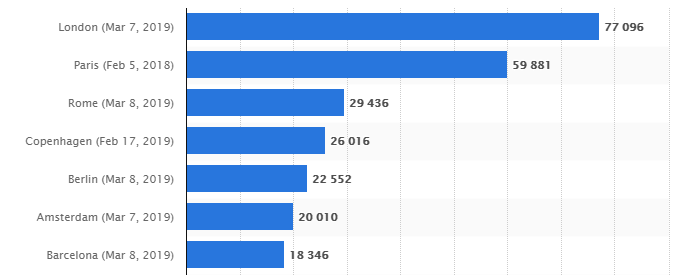
\includegraphics[width=0.8\linewidth]{images/listingplot}
    \caption{\airbnb 2019 new listings}%
    \label{fig:airbnblistingsPlot.PNG}
\end{figure}

When looking at the number of \airbnb listings, we found out that Barcelona, with 18346 listings in 2019, ranked as the seventh European city \cite{europe2019}. As well as the first among Spanish cities. This suggests that Barcelona is one of the biggest \airbnb markets and therefore an interesting way to explore it's revolutionary business model.

Furthermore a study realised in 2013 found out hat \airbnb generated \$175 million in economic activity in one year in Barcelona and supported 4,310 jobs \cite{economy}. As many more users have listed rentals since then, we can only expect that nowadays the amount of jobs and revenue it brings to the city have only increased.

\begin{figure}[H]
    \centering
    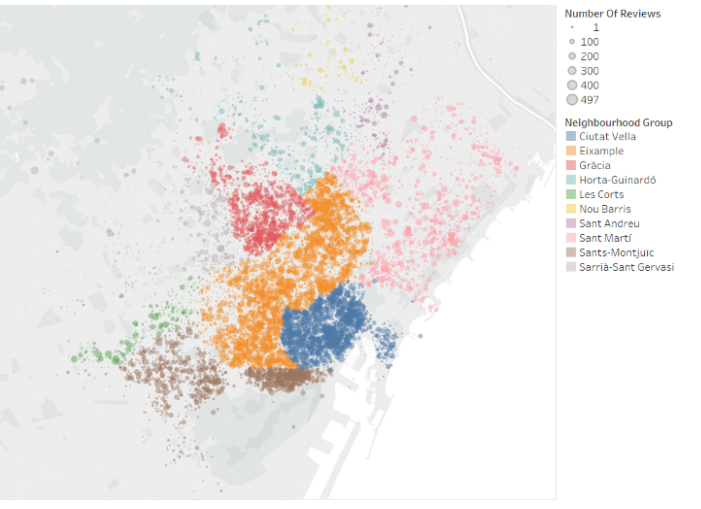
\includegraphics[width=0.8\linewidth]{images/airbnbMap}
    \caption{\airbnb map}%
    \label{fig:airbnbMap.PNG}
\end{figure}

We are specially interested in analysing what makes a successful \airbnb rental. One of the focus of the project will be to analyse whether or not factors such as price, availability or neighbourhood impact whether or not the final user review is positive or negative. 


%% vim: spell spelllang=en:
%! TEX root = **/00-main.tex

% Data Source presentation (repeating what was delivered in first part) (one paragraph)

\section{Data source}%
\label{sec:data_source}

The \airbnb data for Barcelona listings that we use in this project comes from a data
set \cite{dataset} created by Inside AirBnb\footnote{Inside Airbnb: \url{http://insideairbnb.com/}},
which aims to present \airbnb data for most major cities all around the globe in
order to provide valuable insight into how \airbnb is being used in each one of them. It 
extracts this data directly from \airbnb's website and the version of the data set 
we are working with is a snapshot of all Barcelona listings that were available 
on the 24th of August 2020.
%% vim: spell spelllang=en:
%! TEX root = **/00-main.tex


% Formal description of Data structure and metadata

\section{Description of data}%
\label{sec:description_of_data}

% TODO
% What do rows of data matrix contain? (one paragraph)

% Metadata Table

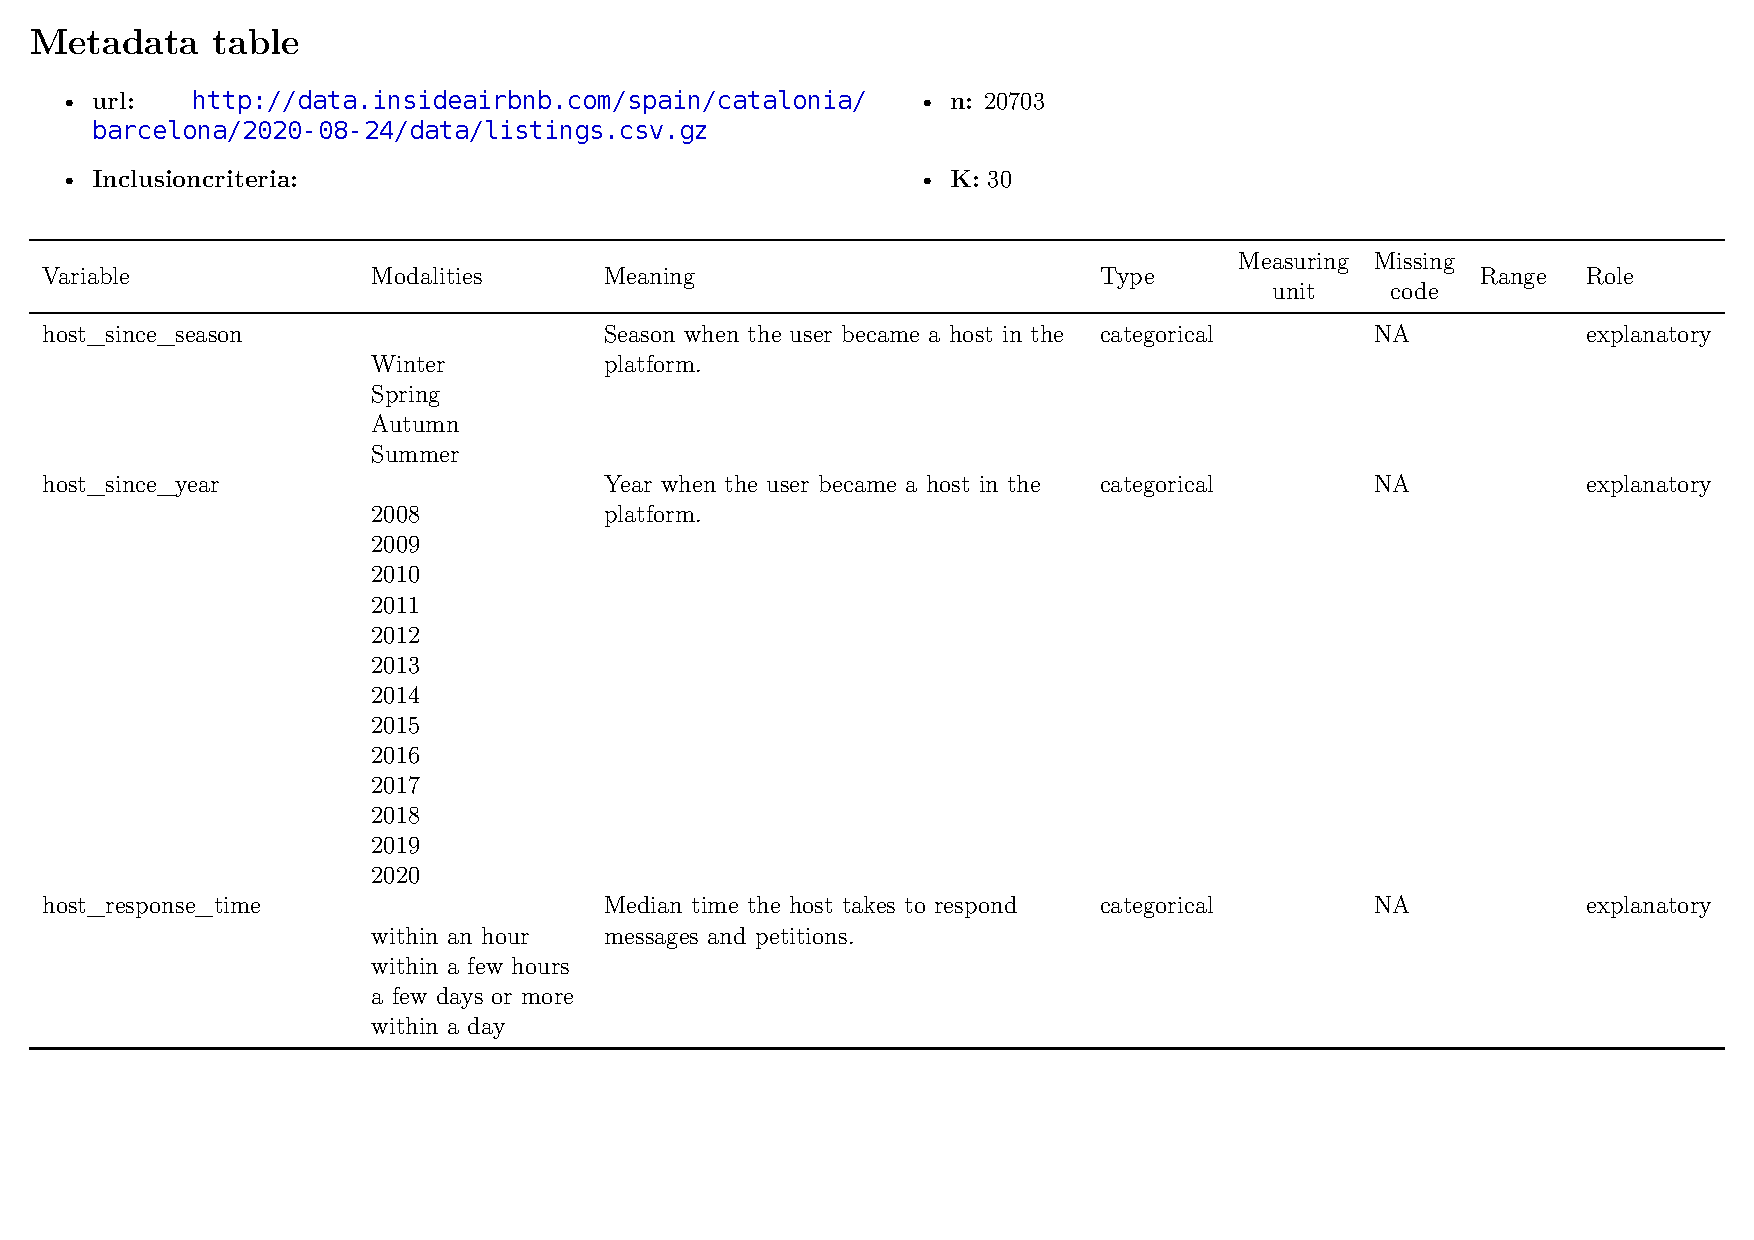
\includepdf[pages=-,landscape=true]{../metadata_table/metadata}

% TODO
% Final scope of the study with inclusion and exclusion criteria for both rows
% and columns (max half a page)

%% vim: spell spelllang=en:
%! TEX root = **/00-main.tex

% Complete Data Mining process performed (one page, including a workflow).

\section{Data mining process}%
\label{sec:data_mining_process}

As discussed in \cref{sec:data_source}, our data came from a single dataset
in \emph{csv} format which we imported in R.

For the initial exploration, we imported the \emph{raw} dataset into R and
inspected the variables provided. Once we had a good understanding of the
variables, their meaning and how they were formated we proceeded with the
preprocessing of the data.

We made several decisions during the preprocessing which are explained in detail
in \cref{sec:preprocessing}. After preprocessing we had a reduced dataset with
a selection of the variables we deemed important for our study.

From the preprocessed dataset we made a more formal statistical description of
the data: a univariate analysis for each variable and bivariate analysis of
various combinations of variables that seemed interesting.

% TODO el NA treatment al final el fem abans o despres de univariate?

The bivariate analysis gave us some insight into the relationships between the
different data columns which gave us some ideas of what to expect in the rest of
the exploratory steps.

For the PCA analysis we tried both the R built-in \texttt{prcomp} function and
the more feature-rich \texttt{PCA} provided by the \texttt{FactoMineR} library.
Although both gave the same results (except for some axis that where reversed),
the \texttt{FactoMineR} library provided more flexibility when representing data
so we used this one.

Similarly, we tried various methods and libraries for the hierarchical
clustering, which are explained in detail in its corresponding section.

\subsection{Workflow}%
\label{sub:workflow}

We decided to create an R script for each process (preprocessing, NA treatment,
PCA, clustering \dots). The data transformation scripts serialize the data frame
which is de-serialized in the other scripts. This makes it so that each script
can be executed independently of the rest without worrying about the current
environment (as long as there is the proper serialized file in the system).

To produce consistent plots we made all scripts share the same function to
export the plots to \emph{pdf} (see script in \cref{sub:shared.r}).

All the scripts used for the project are included in \cref{sec:r_scripts}.

%% vim: spell spelllang=en:
%! TEX root = **/00-main.tex

% Detailed description of Preprocessing and data preparation. Please be sure to
% justify all decisions made.

\section{Preprocessing}%
\label{sec:preprocessing}

% TODO : aixo es copiat tal qual del D3. S'ha de canviar perk sigui el que
%        realment vam acabar fent.

\subsection{Steps and Decisions}%
\label{sub:steps-decisions}

\subsubsection{Formatting issues, building software context}

We haven't encountered any formatting issues or problems with R not recognising
any rows, columns or variable types.

\subsubsection{Determining working matrix}%
\label{ssub:work_matrix}

We discarded many variables from the original data set that didn't provide any
useful information to our project such as URLs and ids or that couldn't be
categorised or were uninteresting such as the \texttt{host\_name}, name and
description of the listing, etc. Furthermore, some columns were duplicated with
different variable names, such as \texttt{host\_listings\_count} and
\texttt{host\_total\_listings\_count}, we removed those redundancies as well.

\subsubsection{Identification and treatment of missing data}

The dataset provided had already all missing data encoded as \NA's. Therefore no
more missing were found encoded as other values. When looking at the missing
values, they appear to be random. Some effort was put into analysing if the missing values had a correlation with the date of the entry, for example if older entries contained more missing data. However we couldn't find any pattern that supported those claims.

Most variables have a missing percentage between 0-5\%. However there are also
variables like \texttt{host\_response\_rate\_cat} with much higher percentages,
reaching up to 35\%. We studied each variable accordingly and performed different missing data treatment techniques.

Categorical with a large number of missing data were analysed and we found out that the best 

Numerical variables were treated using the Knn algorithm. This decision was made because our dataset already contained many numerical variables with no NA's. Therefore Knn seemed the best suited algorithm.

\subsubsection{Identification and treatment of outliers}

When looking at the boxplots of most of the numerical variables in the dataset
we can observe that there are a few outliers. Some of them, although differing
from the general distribution of the values are to be expected. For example the
outliers we find in price, beds or score could easily be explained (maybe they
correlate to the \texttt{room\_type} variable)

On the other hand we also found some outliers that correspond to extreme values
that are not expected. For example in \texttt{maximum\_nights\_avg\_ntm} we
found some rows with the value 2147483647, which corresponds to the maximum
int32 allowed. If we convert that value into years we would get a result that is
unreasonable. After doing some research we found out that the maximum number of nights is limited by AirBnb to 1125. We decided to consider all entries that surpassed that number as errors. 

We have decided to allow for some outliers as long as they are few and
justifiable, in these cases we will try to correlate them to other variables.

\subsubsection{Identification and treatment of errors}

After inspecting the data we have not found errors apart from the one abnormally
large values mentioned before. In those cases we decided to change those values to NA's and then impute those values with the knn algorithm.

\subsubsection{Feature selection/extraction, dimensional reduction}

The \airbnb dataset contained a large amount of variables. First of all we
decided which of them would made it in our working matrix following the steps
detailed in \ref{ssub:work_matrix}. Upon further investigation we decided to
discard additional variables like \texttt{host\_has\_profile\_pic} because the
information it provided wasn't relevant to this project. Of those variables that
made it into our working matrix there are several more relevant than others.

\begin{comment} % TODO posar aixo?

\subsubsection{Instance selection}

\subsubsection{Data transformation}

\end{comment}

\subsubsection{Derivation of new variables}

We derived some new variables from the data set in order to flourish new
categorical variables.

First, starting with the \texttt{host\_since} variable, which gave us the date
the host signed up to \airbnb to list his property, we extracted two new
variables: \texttt{host\_since\_year} and \texttt{host\_since\_season}, both
categorical. \texttt{host\_since\_year} categorizes the host sign up dates into
their particular year and since. The variable \texttt{host\_since\_season}
represents the season of the year during which the host signed up. For the
latter, the modalities are Winter, Spring, Summer and Autumn.

We have also categorized \texttt{host\_response\_rate} and
\texttt{host\_acceptance\_rate} as we converted them from a numerical variables
measured in percentages to categorical ones with the following modalities: very
low, low, average, high and very high.

These were all the variable derivations we carried out in our data set for this
project. They were all motivated by the necessity to have more categorical
variables in our data set, as it had plenty numerical and binary variables but
was short of categorical ones.

% Enumerate which steps of the preprocessing process are used with your
% particular data (consider the steps proposed in slide 4 of Preprocessing
% Slides in Theme 2. Data Preparation. Remember that you have the whole complete
% information on preprocessing in the reference text from the linkSurvey of
% preprocessing. Reference paper (MIE 2001) from complementary materials section
% of Theme 2. Data Preparation)

% List and justify all decisions taken for each preprocessing step

% Additional descriptive statistics of variables that have been modified or
% created by preprocessing

%% vim: spell spelllang=en:
%! TEX root = **/00-main.tex

\newcommand{\sssfig}[1]{
    \pagebreak
    \subsubsection{#1}%
    \label{ssub:#1}
}

\newcommand{\hibp}[2]{
    \begin{figure}[H]
        \centering
        \includegraphics[width=0.8\linewidth]{desc-#1-hi_bp}
        \caption{Histogram \& Boxplot of #2}%
        \label{fig:#1}
    \end{figure}
}

\newcommand{\tabn}[2]{
    \begin{table}[H]
        \centering
        \caption{Extended summary statistics of #2}%
        \label{tab:#2}
        \input{../../analysis/tables/desc-#1-ext_sum}
    \end{table}
}

\newcommand{\fign}[2]{
    \sssfig{#2}
    \hibp{#1}{#2}
    \tabn{#1}{#2}
}

\newcommand{\figf}[2]{
\sssfig{#2}
\begin{figure}[H]
    \begin{minipage}{0.49\linewidth}
            \centering
            \includegraphics[width=\linewidth]{desc-#1-bar}
    \end{minipage}
    \begin{minipage}{0.49\linewidth}
            \centering
            \includegraphics[width=\linewidth]{desc-#1-pie}
    \end{minipage}
    \caption{Barplot \& Pie chart of #2}%
    \label{fig:#1}
\end{figure}
\begin{table}[H]
    \centering
    \caption{Table of #2 frequency}%
    \label{tab:#1}
    \input{../../analysis/tables/desc-#1-freq}
\end{table}
}

% Basic statistical descriptive analysis

\section{Basic statistical descriptive analysis}%
\label{sec:basic_statistical_descriptive_analysis}

% Univariate for all the variables included in the study (half a page per variable)
\subsection{Univariate analysis}%
\label{sub:univariate_analysis}

%\begin{comment}

\begin{table}[H]
    \centering
    \caption{Numerical variables summary}%
    \label{tab:num_summary}
    \resizebox{\linewidth}{!}{%
    
\begin{tabular}[t]{llllllll}
\toprule
  & Min & 1st Q. & Median & Mean & 3rd Q. & Max & NA's\\
\midrule
host\_listings\_count & 0.00 & 1.00 & 2.00 & 16.81 & 11.00 & 551.00 & 8\\
accommodates & 1.000 & 2.000 & 2.000 & 3.297 & 4.000 & 16.000 & NA\\
bedrooms & 1.000 & 1.000 & 1.000 & 1.604 & 2.000 & 16.000 & 684\\
beds & 0.000 & 1.000 & 2.000 & 2.233 & 3.000 & 48.000 & 409\\
price & 0.00 & 35.00 & 55.00 & 86.34 & 95.00 & 10000.00 & NA\\
\addlinespace
minimum\_nights\_avg\_ntm & 1.00 & 1.40 & 2.70 & 10.67 & 12.10 & 1123.00 & NA\\
maximum\_nights\_avg\_ntm & 1.000e+00 & 3.300e+02 & 1.125e+03 & 3.118e+05 & 1.125e+03 & 2.147e+09 & NA\\
availability\_30 & 0.00 & 0.00 & 24.00 & 17.55 & 30.00 & 30.00 & NA\\
availability\_60 & 0.00 & 0.00 & 52.00 & 36.43 & 59.00 & 60.00 & NA\\
availability\_90 & 0.00 & 3.00 & 80.00 & 56.01 & 89.00 & 90.00 & NA\\
\addlinespace
availability\_365 & 0.0 & 55.0 & 180.0 & 191.3 & 352.0 & 365.0 & NA\\
number\_of\_reviews & 0.0 & 0.0 & 5.0 & 33.1 & 36.0 & 743.0 & NA\\
number\_of\_reviews\_ltm & 0.000 & 0.000 & 1.000 & 6.401 & 9.000 & 278.000 & NA\\
number\_of\_reviews\_l30d & 0.0000 & 0.0000 & 0.0000 & 0.1621 & 0.0000 & 15.0000 & NA\\
review\_scores\_rating & 20.00 & 88.00 & 93.00 & 91.08 & 98.00 & 100.00 & 5971\\
\addlinespace
review\_scores\_accuracy & 2.000 & 9.000 & 10.000 & 9.379 & 10.000 & 10.000 & 5982\\
review\_scores\_cleanliness & 2.000 & 9.000 & 9.000 & 9.227 & 10.000 & 10.000 & 5980\\
review\_scores\_location & 2.000 & 9.000 & 10.000 & 9.618 & 10.000 & 10.000 & 5985\\
review\_scores\_value & 2.000 & 9.000 & 9.000 & 9.055 & 10.000 & 10.000 & 5985\\
reviews\_per\_month & 0.010 & 0.210 & 0.710 & 1.179 & 1.770 & 21.410 & 5731\\
\bottomrule
\end{tabular}
}
\end{table}

\Cref{tab:num_summary} shows an overview of the numerical variables statistics.


\fign{accommodates}{Accommodates}
% Use this to not pagebreak from subsection

%\subsubsection{Accommodates}%
%\label{ssub:accommodates}
%\hibp{accommodates}{Accommodates}
%\tabn{accommodates}{Accommodates}

In the boxplot we can that there are some outliers. However the distribution of
the variable seems to be in line with socioeconomic distributions. The majority
of listing have low to medium capacities (small-medium houses), while there's
only a fraction of high capacities (big houses).


\fign{bedrooms}{bedrooms}

The majority of listing contains between 1-4 bedrooms, being the mean around
1.6. There are some outliers, but they can somewhat be explained due to the same
reasons mentioned in the accommodates analysis.


\fign{beds}{beds}

The distribution of beds and the outliers seem to follow a similar distribution
as bedrooms.  This is to be expected as those to variables should be correlated.


\fign{availability_30}{availability 30}

If we look at the availability in the next 30 days after the data was taken, we
can clearly see some polarization. There are some rentals with 0 available days
and some close to all days. This polarization explains the high variance of this
variable.


% TODO: ho posem a l apendix?
%\fign{availability_60}{availability 60}
%\fign{availability_90}{availability 90}
\fign{availability_365}{availability 365}

The availability of the year follows a similar distribution to the monthly one.
The only difference are some peaks at 90 days and half a year, which both are
likely numbers for a host to rent its listing.


\figf{host_acceptance_rate_cat}{host acceptance rate cat}

Up to 66\% of the hosts have a very high chance of accepting a customer. There
is a large number of \emph{NA}'s as well.


\figf{host_has_profile_pic}{host has profile pic}

As seen in \cref{fig:host_has_profile_pic}, over 99\% of host with
listings in Barcelona have a profile picture, in fact only 55 out of 20,476
hosts don't have a picture. Therefore, we don't expect this variable to provide
significant insight into answering the question we are posing.

\figf{host_identity_verified}{host identity verified}

\Cref{fig:host_identity_verified} shows that only 74\% of hosts have had
their identity verified by \airbnb, meaning that the other 25\% isn't.  This can
be expected since the verification process can be complicated in some cases,
even requiring the host to provide an official document or additional pictures
of himself.

\figf{host_is_superhost}{host is superhost}

As seen in \cref{fig:host_is_superhost}, only the 19\% of hosts are superhosts.
This may be the case because the conditions to achieve this status are rather hard.

\fign{host_listings_count}{host listings count}


\Cref{fig:host_listings_count} shows that the majority of hosts only have a
small amount of listings, being the median 2. However we can see that there is a
lot of variability with many outliers. These outliers might correspond to
businesses that own lots of listings.

% TODO
%\fig{desc-host_listings_count-hi_bp-tallat100}{host listings count}


\figf{host_response_rate_cat}{host response rate cat}

This variable conveys how attentive the host is, as it tells us to what degree
the host replies to messages received inquiring about its listings. As seen in
\cref{fig:host_response_rate_cat}, 55\% of hosts have a very high
response rate, that is they reply to more than 80\% of messages they receive.
It should be noted that this variable has a high share of missing data,
approximately 34\%.


\figf{host_response_time}{host response time}

\Cref{fig:host_response_time} shows that the quicker the response, the more
number of entries it has. A fact to point out as well is the large number of
\emph{NA}'s.


\figf{host_since_season}{host since season}

To our surprise there number of new hosts listings remain more or less equal over
the four seasons. In \cref{fig:host_since_season} we can see that Spring/Summer
still have a bigger influx but not as much as we had initially hypothesised.


\figf{host_since_year}{host since year}

In \cref{fig:host_since_year} we can see that except for the first years the
among of new hosts has more or less remained constant. However in 2019 there has
been another spike of new hosts.


\figf{instant_bookable}{instant bookable}

As seen in \cref{fig:instant_bookable} there are nearly as many
instant bookable listings as not.

%\end{comment}

% TODO

%\fign{maximum_nights_avg_ntm}{maximum nights avg ntm}

%\fig{maximum_nights_avg_ntm-hi_bp-post}{maximum nights avg ntm post}

%\fign{minimum_nights_avg_ntm}{minimum nights avg ntm}

\figf{neighbourhood_group_cleansed}{neighbourhood group cleansed}

Looking at \cref{fig:neighbourhood_group_cleansed} we can see that
L'Eixample and Ciutat Vella are the most popular neighborhoods for listing.


\fign{price}{price}
\fig{desc-price-hi_bp-tallat500}{price}

In \cref{fig:desc-price-hi_bp-tallat500} we can see that there are some extreme
outliers. To visualize the distribution better we have cut the histogram at
price 500. Having done that we can see that the price distribution seems to
follow a chi-square. We were surprised to find out that the mean price is around
\$86.34.


\fign{review_scores_rating}{review scores rating}

We can see that the majority of reviews are considered positive. The mean in
fact is a 91.07. That would explain why a common technique among renters is to
consider any review lower than 90 as negative.

We can see as well that there is some polarization, being the most common rating
among negative reviews a 0 and the most common among positive a 10. We suppose
polarization occurs because users are more likely to leave reviews when they had
either really good or really bad experiences.


\fign{review_scores_value}{review scores value}

This variable follows a similar distribution as the other reviews seen so far.
Despite that it has the peculiarity of having less perfect scores.


\fign{review_scores_location}{review scores location}

The location score seems to be the one with most positive reviews. In fact the
mean is 9.61, almost 0.5 higher than the overall rating. We found as well very
few negative reviews, being in fact the median and Q3 both a 10.


\fign{review_scores_accuracy}{review scores accuracy}

The distribution of this variable is really similar to the review score ratings.


\fign{review_scores_cleanliness}{review scores cleanliness}

The distribution of this variable is really similar to the review score ratings.


% TODO

\fign{number_of_reviews}{number of reviews}
\fign{number_of_reviews_l30d}{number of reviews l30d}
\fign{number_of_reviews_ltm}{number of reviews ltm}

\fign{reviews_per_month}{reviews per month}

When looking at \cref{fig:reviews_per_month} we can clearly see a decreasing
curve with its mean around 1.17. We found some outliers with the max number of
reviews per month being 21. Despite it being quite larger than the mean we think
it is still plausible to have 21 reviews over a 30 day span.

\figf{room_type}{room type}

The vast majority of listings correspond to entire homes/apartments or private
rooms.

\pagebreak
% Bivariate when relevant (half a page per pair of variables)
\subsection{Bivariate analysis}%
\label{sub:bivariate_analysis}

\subsubsection{Host since year vs host listings count}

\fig{bivar-host_since_year-host_listings_count}{Number of listings depending on the year the host joined Airbnb}



Looking at \cref{fig:bivar-host_since_year-host_listings_count} we can see that
there is no clear correlation between the number of listings a host has and the
time they have been in the platform.It seems like most of the users have a small
amount of listings.

However, the small group that joined the platform in the years 2009, 2010 and
2011 seems to include some owners with upwards of 100 and 150 listings. This
seems to confirm that most of the early adopters of the platform were businesses
or big owners that gathered a lot of buildings. We can also see that some of the
hosts with more listings joined in the recent years, probably joining the
platform after seeing great results from others' operations.


\pagebreak
\subsubsection{Host since year vs price per night}

\fig{bivar-host_since_year-price}{Price per night depending on the year the host joined \airbnb}

Looking at \cref{fig:bivar-host_since_year-price} we can see that again, there
is no relation between the price of the listings and the year the host joined,
there are a few differences on price, all in the neighbourhood of 80-125 dollars
a night, but we also see the same tendency we saw in the last graph, the median
price for the listings posted by hosts who joined during years 2009, 2010 and
2011 seems to be a bit higher than the median price for the hosts who joined in
subsequent years.

\pagebreak

\subsubsection{Host since year vs room type}

\fig{bivar-host_since_year-room_type}{Room type depending on the host's joining year}


What we wanted to find out with \cref{fig:bivar-host_since_year-room_type} was
if there was any initial promotion within a certain group of hosts, something
along the lines of contacting different hotel chains to promote the platform,
which at that time was still small, and give them certain advantages to use
\airbnb.
We would have expected, if that was the case, a significantly bigger share of
the early years' hosts to be listing hotel rooms instead of private rooms or
entire apartments.
This obviously was not the case, which is interesting, since it indicates that
\airbnb did not grow through the kind of techniques we had expected.


\pagebreak
\subsubsection{Number of reviews vs review score rating}

\fig{bivar-number_of_reviews-review_scores_rating}{Score rating vs number of reviews}

 In this case, \cref{fig:bivar-number_of_reviews-review_scores_rating} shows how
 the number of reviews affects the total rating. We can see that when there are
 not many reviews those can be anywhere within range, but once the listings get
 a significant amount of reviews it is harder and harder to find listings with a
 low rating. This, we believe, is due to people's tendency to give polarized
 scores and avoid booking the listings with really low scores.

\pagebreak
\subsubsection{Reviews per month vs review score rating vs price}

\fig{bivar-reviews_per_month-review_scores_rating}{Score rating vs reviews per month}

 To see if there is a difference, we have created
 \cref{fig:bivar-reviews_per_month-review_scores_rating}, which shows how the
 number of reviews per month correlates to the score of the reviews a listing
 has, but also integrating the price of such listing. It is interesting to see
 that some of the most reviewed listings are not very expensive and that the
 tendency that we saw in \cref{fig:bivar-host_since_year-room_type} is still
 there, proving that the listings that get reviewed the most tend to have pretty
 good ratings.

\pagebreak

\fig{bivar-price-neighbourhood_group_cleansed}{Price of listings depending on the neighbourhood \airbnb}

% TODO: Nose si a la figure "we can see" els mean prices XD
As Barcelona dwellers we know that there are some neighborhoods more expensive
to others. We want to find out if this still holds when talking about \airbnb
rents.  We can see in figure \cref{fig:bivar-price-neighbourhood_group_cleansed}
that for example L'Eixample has a mean price of 96.20, %TODO dollars / euros?
while Nou Barris has a mean price of 41.10.  %TODO dollars / euros?
We can see as well that the high price outliers seem to vary between
neighborhoods. This leads us to believe that although not much there is some
correlation between price and neighborhood.

\pagebreak

\fig{bivar-room_type-minimum_nights_avg_ntm}{Minimum number of nights depending on room type}

From figure \cref{fig:bivar-room_type-minimum_nights_avg_ntm} we can clearly see
that hotel rooms and shared rooms have a minimum average of nights much lower
than the entire homes or private rooms.  We can see that entire homes/apartments
have less variance, being the majority of values concentrated near the mean,
while in the private rooms we can see a much larger interquartile range.

% When required, please include descriptives before and after preprocessing
\subsection{Conclusion}%
\label{sub:data-conclusion} % TODO


% Conclude the section with one paragraph describing how is your data

%% vim: spell spelllang=en:
%! TEX root = **/00-main.tex

% PCA analysis for numerical variables:

\section{PCA analysis for numerical variables}%
\label{sec:pca_analysis_for_numerical_variables}

% Scree plot. Specify how many principal components are selected
\subsection{Scree plot}%
\label{sub:scree_plot}


\begin{figure}[H]
    \centering
    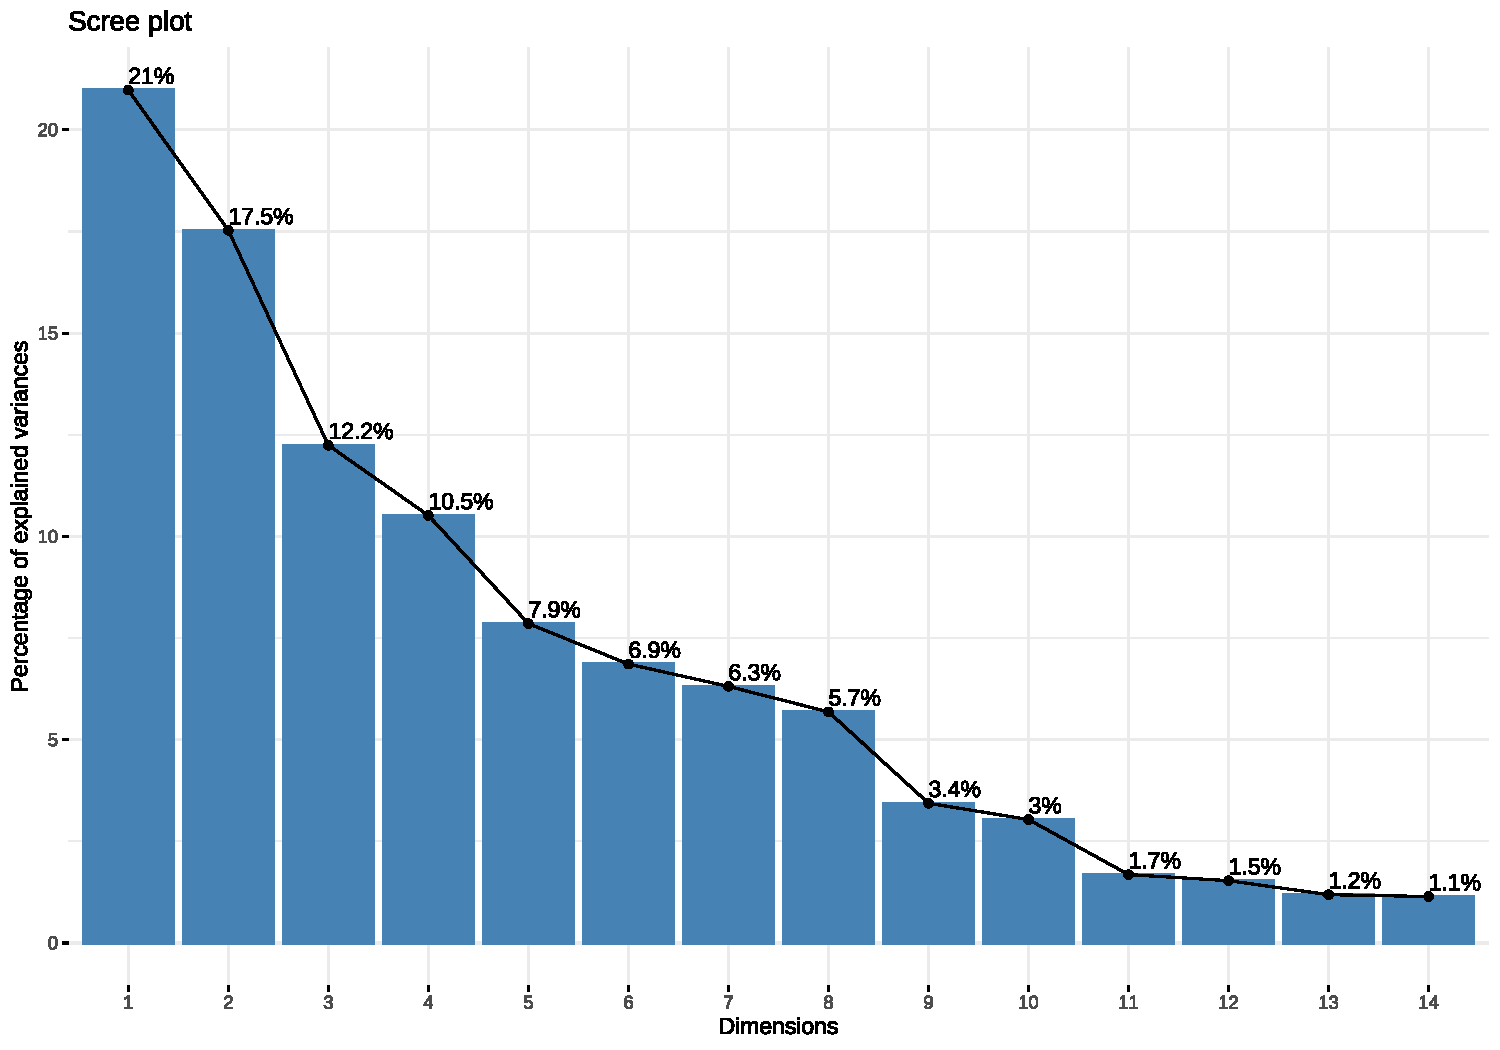
\includegraphics[width=0.7\linewidth]{pca_fact-screeplot} % PCA-inertia_cum
    \caption{PCA inertia}%
    \label{fig:pca_inertia}
\end{figure}

\begin{figure}[H]
    \centering
    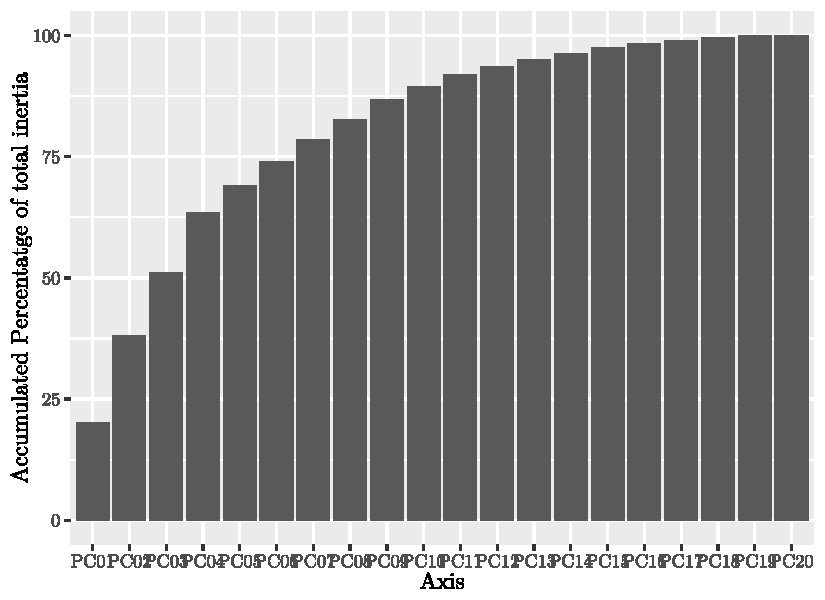
\includegraphics[width=0.7\linewidth]{PCA-inertia_cum}
    \caption{PCA accumulated inertia}%
    \label{fig:pca_inertia_cum}
\end{figure}

\vspace{-1em}
We used the inertia plots to decide the number of factorial axis to analyse. In
\cref{fig:pca_inertia} we can conclude the 4 first axis represent a much
larger amount of variance compared to the others. When looking at
\cref{fig:pca_inertia_cum} we can see that the first 4 axis already contain 63\%
of the variance. If we analyse further with the elbow method we can clearly see
that the slop starts to decrease at around the 4\ts{th} axis. Therefore we decided to
only further analyse the first 4 factorial axis.

% 20.24968405 17.88042469 13.04514781 12.39547495
% 20.24968  38.13011  51.17526  63.57073     %  69.09301  74.04671  78.51992  82.73880

\begin{table}[H]
    \centering
    \caption{Eigenvalues \& variance percentage of first 5 Dimensions}%
    \label{tab:eig}
    
\begin{tabular}[t]{lrrr}
\toprule
  & Eigenvalue & Var. \% & Cum. Var. \%\\
\midrule
comp 1 & 4.0499368 & 20.249684 & 20.24968\\
comp 2 & 3.5760849 & 17.880425 & 38.13011\\
comp 3 & 2.6090296 & 13.045148 & 51.17526\\
comp 4 & 2.4790950 & 12.395475 & 63.57073\\
comp 5 & 1.1044548 & 5.522274 & 69.09301\\
\addlinespace
comp 6 & 0.9907408 & 4.953704 & 74.04671\\
comp 7 & 0.8946421 & 4.473211 & 78.51992\\
comp 8 & 0.8437760 & 4.218880 & 82.73880\\
comp 9 & 0.8078400 & 4.039200 & 86.77800\\
comp 10 & 0.5511517 & 2.755759 & 89.53376\\
\bottomrule
\end{tabular}
\end{table}

\begin{table}[H]
    \centering
    \caption{Variable contribution to each axis}%
    \label{tab:}
    
\begin{tabular}[t]{lrrrr}
\toprule
  & Dim.1 & Dim.2 & Dim.3 & Dim.4\\
\midrule
host\_listings\_count & 1.1978839 & 0.2309859 & 1.2348477 & 1.9194330\\
accommodates & 1.7298781 & 4.9204820 & 15.4579382 & 8.8411427\\
bedrooms & 1.5035858 & 3.8248072 & 14.2067930 & 10.2701716\\
beds & 1.5539744 & 4.1550603 & 14.5044651 & 9.4446670\\
price & 0.3358423 & 0.5034663 & 1.7979068 & 2.5310976\\
\addlinespace
minimum\_nights\_avg\_ntm & 0.3285224 & 0.1053913 & 0.8458848 & 1.3083557\\
maximum\_nights\_avg\_ntm & 0.0326754 & 0.1551460 & 0.0180542 & 0.1915016\\
availability\_30 & 4.7100532 & 13.9585375 & 7.7416460 & 0.0782981\\
availability\_60 & 5.0921343 & 15.0338778 & 8.3809077 & 0.0804272\\
availability\_90 & 5.0164904 & 15.0703072 & 8.1727252 & 0.0732742\\
\addlinespace
availability\_365 & 3.9814077 & 9.6538067 & 2.9478169 & 0.0828489\\
number\_of\_reviews & 1.3671328 & 5.0656577 & 6.0696363 & 12.6128426\\
number\_of\_reviews\_ltm & 1.4742472 & 5.9390691 & 6.6049015 & 15.9807855\\
number\_of\_reviews\_l30d & 0.3293267 & 1.6735082 & 1.7305596 & 5.7081947\\
review\_scores\_rating & 16.2922433 & 2.7642390 & 1.0363407 & 3.3113763\\
\addlinespace
review\_scores\_accuracy & 15.2310328 & 2.7062625 & 0.7857840 & 2.4644208\\
review\_scores\_cleanliness & 12.6689566 & 3.1473241 & 0.5491346 & 2.7145276\\
review\_scores\_location & 9.5058782 & 2.5671720 & 0.4498178 & 1.7099762\\
review\_scores\_value & 15.7847912 & 2.5825171 & 1.1601061 & 2.4687109\\
reviews\_per\_month & 1.8639432 & 5.9423821 & 6.3047340 & 18.2079477\\
\bottomrule
\end{tabular}
\end{table}

% Factorial map visualisation:
\subsection{Factorial map visualisation}%
\label{sub:factorial_map_visualisation}

% #2 -> caption #3 -> file, #1 -> page
\newcommand{\factorialmap}[2]{
    \begin{landscape}
    \begin{figure}[H]
        \centering
        \includegraphics[width=0.87\linewidth]{pca_fact-plane_#1_#2-bi}
        \caption{PCA plane #1 vs #2}%
        \label{fig:plane_#1-#2}
    \end{figure}
    \end{landscape}
}

\newcommand{\factvar}[2]{
    \begin{figure}[H]
        \centering
        \includegraphics[width=0.67\textwidth]{pca_fact-plane_#1_#2-var}
        \caption{PCA plane #1 vs #2 (numerical)}%
        \label{fig:plane_#1-#2-var}
    \end{figure}
}

\newcommand{\factorialmapCV}[2]{
    \contrib{#1}{#2}
    \factvar{#1}{#2}
}

\newcommand{\contrib}[2]{
    \begin{figure}[H]
        \centering
        \includegraphics[width=0.85\linewidth]{pca_fact-plane_#1_#2-contrib}
        \caption{PCA variable contributions of plane #1 vs #2}%
        \label{fig:contrib_plane_#1-#2}
    \end{figure}
}

\newcommand{\categorica}[4]{
    \begin{figure}[H]
        \centering
        \includegraphics[width=0.85\linewidth]{pca_fact-#3-plane_#1_#2}
        \caption{PCA variable contributions of #4 in plane #1 vs #2}%
        \label{fig:cat-#3-plane-#1-#2}
    \end{figure}
}

%TODO

\factorialmap{1}{2}
In \cref{fig:plane_1-2} we are showing the factorial maps that represent the most variance among all our factorial axis. When looking at the numerical variables represented we can see that all there are some variables that tend to be grouped. For example
there's a group about all review scores, another with beds, bedroom and accommodates and another with availabilities. When 
analysing \cref{fig:contrib_plane_1-2} we can see that accommodates, beds and the review scores are top contributors to
this plane. When analysing the contribution to each plane it's clear that review scores are affecting mostly axis 2, whereas accommodates and beds mostly affect axis 1.

\begin{comment}
In \cref{fig:plane_1-2} we are showing the factorial maps that represent the most variance among all our factorial axis. When looking at the numerical variables represented we can see that all the variables
related to reviews tend to have similar arrows, this makes sense 
because in the bivariate analysis we concluded that they were correlated.
Looking at \cref{fig:contrib_plane_1-2} we can see that the variables
with higher contribution are the ones about review scores and availability. As all review score variables have a small angle to the first factorial axis we can begin to speculate that this axis is 
mostly affected by these variables. Other variables like availability
and accommodates seem to contribute mostly to the second factorial axis, however these angles aren't as tight so they probably affect the first axis as well. 
\end{comment}
\factorialmapCV{1}{2}


\factorialmap{1}{3}
In \cref{fig:plane_1-3} we can see that it seems to hold true that the accommodates and beds affects axis 1 the most. Price 
seems to have a similar arrow as those variables. This might be
because there is some correlation between those variables. 
(The more beds a house has, probably the more expensive it is).
The arrows of variables about number of reviews have a very small angle with factorial axis 3. Minimum\_nights\_avg\_ntm seem to
be affecting axis 3 as well but inversely.

\factorialmapCV{1}{3}

\factorialmap{1}{4}

In \cref{fig:plane_1-4} we can see that again it is true
the accommodates and beds variables affects axis 1 the most. We can begin to speculate that these might be factorial axis 1
latent variables. Looking at \cref{fig:contrib_plane_1-4} we 
can see that availabities first appear as top contributors and seem to be related with the forth factorial axis.

\begin{comment}
The plane in \cref{fig:plane_1-4} seems to be mostly affected by review scores and the number of reviews.
In this specific plane number of reviews and accommodates seem to have a similar contribution but with
inverse relation. We can maybe relate the availability with the first plane, but as the global correlation
to this plane of this variable isn't has high we can't derive to much from this.
\end{comment}

\factorialmapCV{1}{4}


\factorialmap{2}{3}
%TODO
In \cref{fig:contrib_plane_2-3} the most contributing variables are the availabilities, accommodates and bedrooms.
These particular plot doesn't help us much in regards to finding associations with the axis because the
angles the variables form are too wide.
\factorialmapCV{2}{3}


\factorialmap{2}{4}

What we can extract when analysing \cref{fig:plane_2-4} is that the availability variables have 
a relatively high contribution and form a very small angle with the forth factorial axis. The same happens with review scores and the second axis.

\factorialmapCV{2}{4}


\factorialmap{3}{4}
We can't extract much more from \cref{fig:plane_3-4}. Everything
aforementioned seems to hold true in this specific plane.

\factorialmapCV{3}{4}

\begin{landscape}

\categorica{1}{2}{room_type}{room type}
\categorica{1}{3}{room_type}{room type}
\categorica{1}{4}{room_type}{room type}

\end{landscape}

\subsection{Conclusion}%
What we can conclude after analysing how the variables are distributed along each factorial axis is 
that our variables generally distribute in 4 groups: the ones about availability, 
the ones about review scores, the ones regarding number of reviews and finally beds and accommodation. That might happen
because there is some correlation between them.

After studying each factorial axis in depth we can concluded that the latent variables associated to 
the first factorial map are the ones that talk about review scores. We reached these conclusion after
seeing that in all PCA plots with with the first factorial axis, these variables were top contributors
and their angles to the first axis were really small. The relation seems to be direct as in all plots 
they appear in the positive first axis. Although this relation appears in all plots where factorial
axis 1 appears we think \cref{fig:plane_1-3} depicts this relation the best. 

We conclude that the PCA visualization was an overall success because we were able to detect some grouped
variables and relate some of them to our factorial axis. In fact, we ended up associating the first axis
with the review score variables. This is a major success because the first factorial axis is the one
that represents more variance and therefore associating a meaning to it could help us better explain
out variables.


% (Be sure you use a single landscape pager for each single map in order to
% guarantee visibility of materials to the readers)

% For each factorial map provide:

% - Individuals projections

% - Common projection of numerical variables and modalities of qualitative
% - variables (take care to use correct color codes as explained along the course)

% - Interpretation of relationships among variables observed. When possible,
% - interpret the latent variable associated with the principal axis

% - Conclusions

% Note: All factorial maps must be placed in a single landscape page that makes
% it visible

%% vim: spell spelllang=en:
%! TEX root = **/00-main.tex

% Hierarchical Clustering on original data:

\section{Hierarchical Clustering}%
\label{sec:hierarchical_clustering}

\subsection{Description of data}%
\label{sub:description_data}
% TODO:

% Precise description of the data used (which variables have not been included
% in the analysis, if any, whenever you are using a CURE strategy, provide
% details about eventual sampling performed on data, etc)

We decided to investigate two different hierarchical clustering methods to
identify which one worked best with our data set: Ward's hierarchical method and 
Hierarchical Clustering on Principal Components (HCPC). Ward uses
the whole preprocessed data set while HCPC uses the PCA outcome. None of the
methods required any kind of sampling.

\subsection{Methods and metrics}

% Clustering method used, metrics and aggregation criteria used (Ward’s method
% is recommended embedded or not in a CURE strategy whenever scaling to big data
% is required, for messy data Gower dissimilarity coefficient to the square is
% recommended )

As mentioned in \ref{sub:description_data}, we explored two different clustering methods.
ward.D and ward.D2 both use Ward's hierarchical method, but 


\begin{figure}[H]
    \centering
    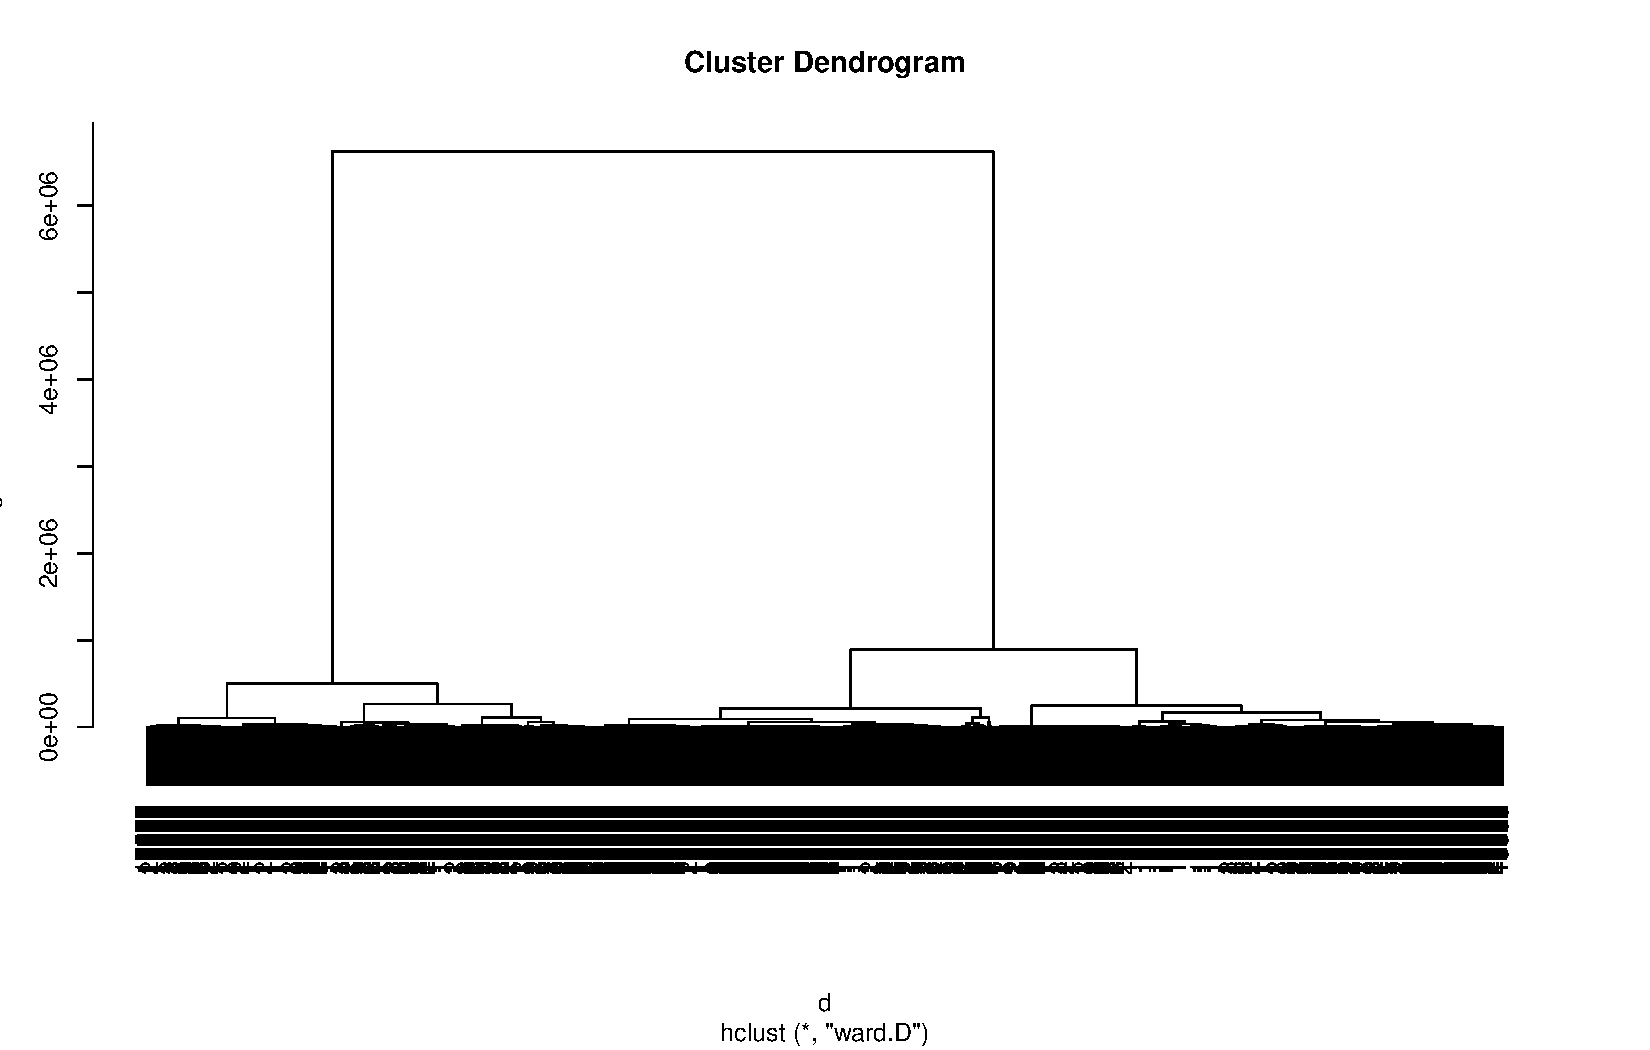
\includegraphics[width=0.8\linewidth]{cluster-dendo-h1}
    \caption{Cluster Dendogram}%
    \label{fig:dendogram}
\end{figure}

\begin{figure}[H]
    \centering
    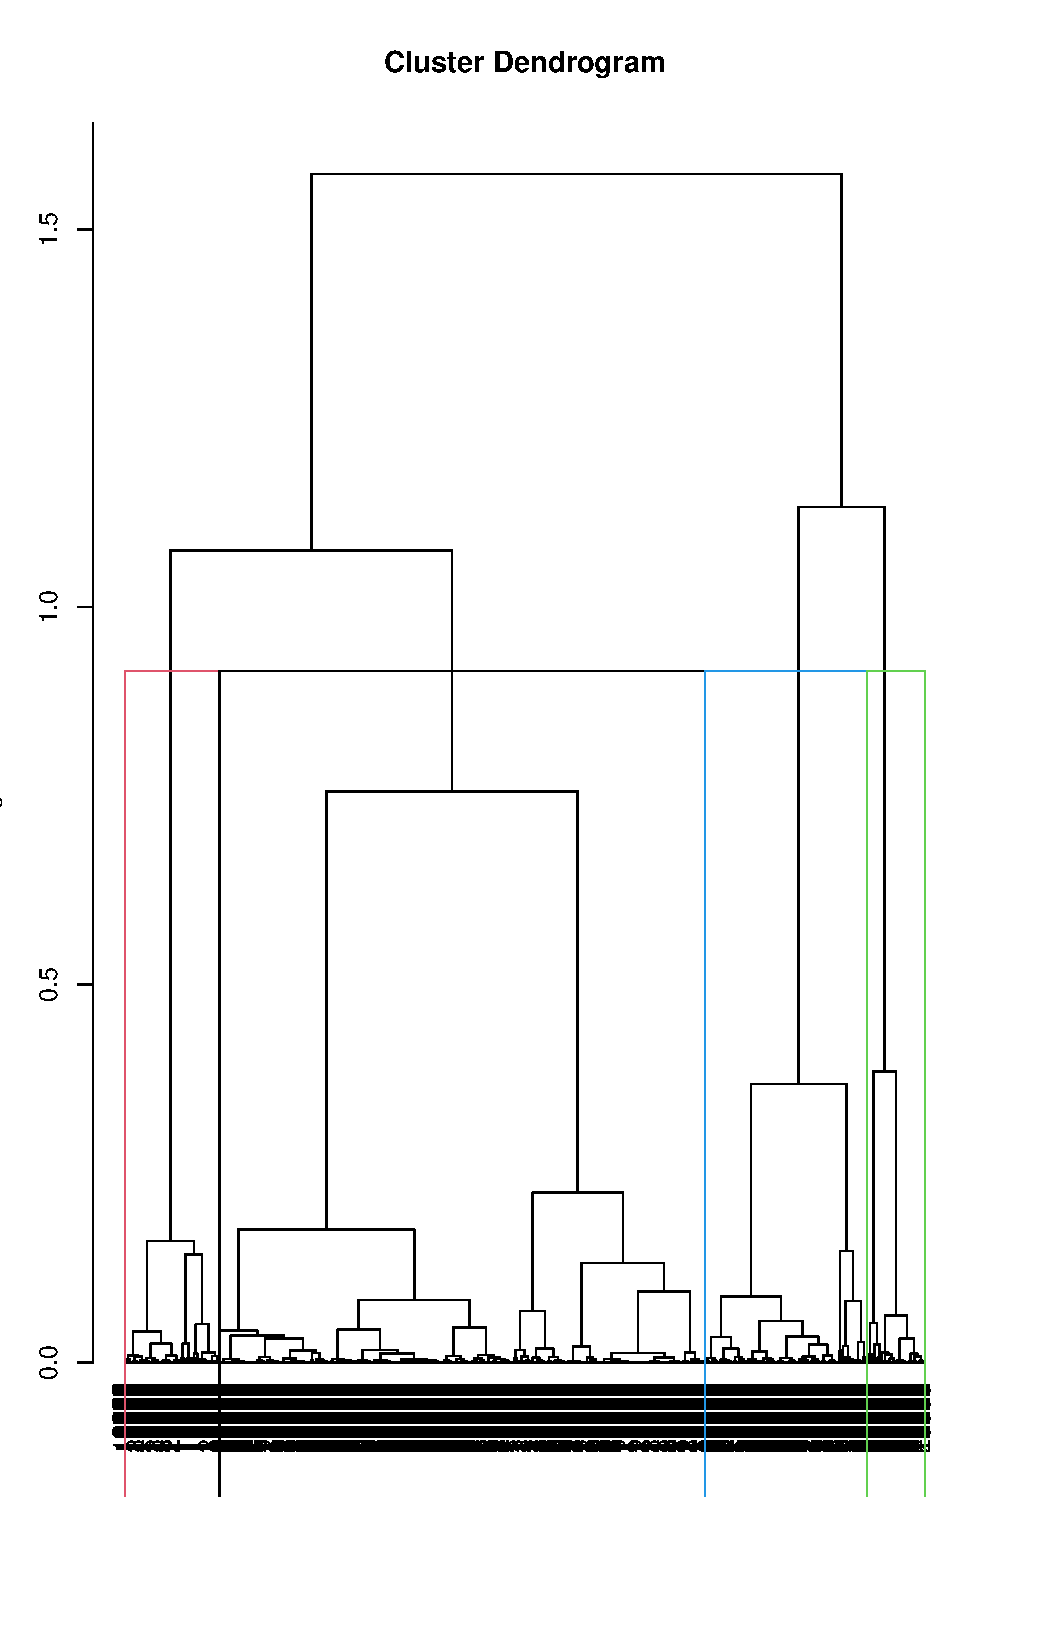
\includegraphics[width=0.8\linewidth]{cluster-dendo-h3}
    \caption{Cluster Dendogram}%
    \label{fig:dendogram}
\end{figure}

\begin{landscape}

\subsection{Dendogram}%
\label{sub:dendogram}

% Resulting Dendrogram (of the total dataset or the sample). USE A SINGLE PAGE
% for it

\begin{figure}[H]
    \centering
    %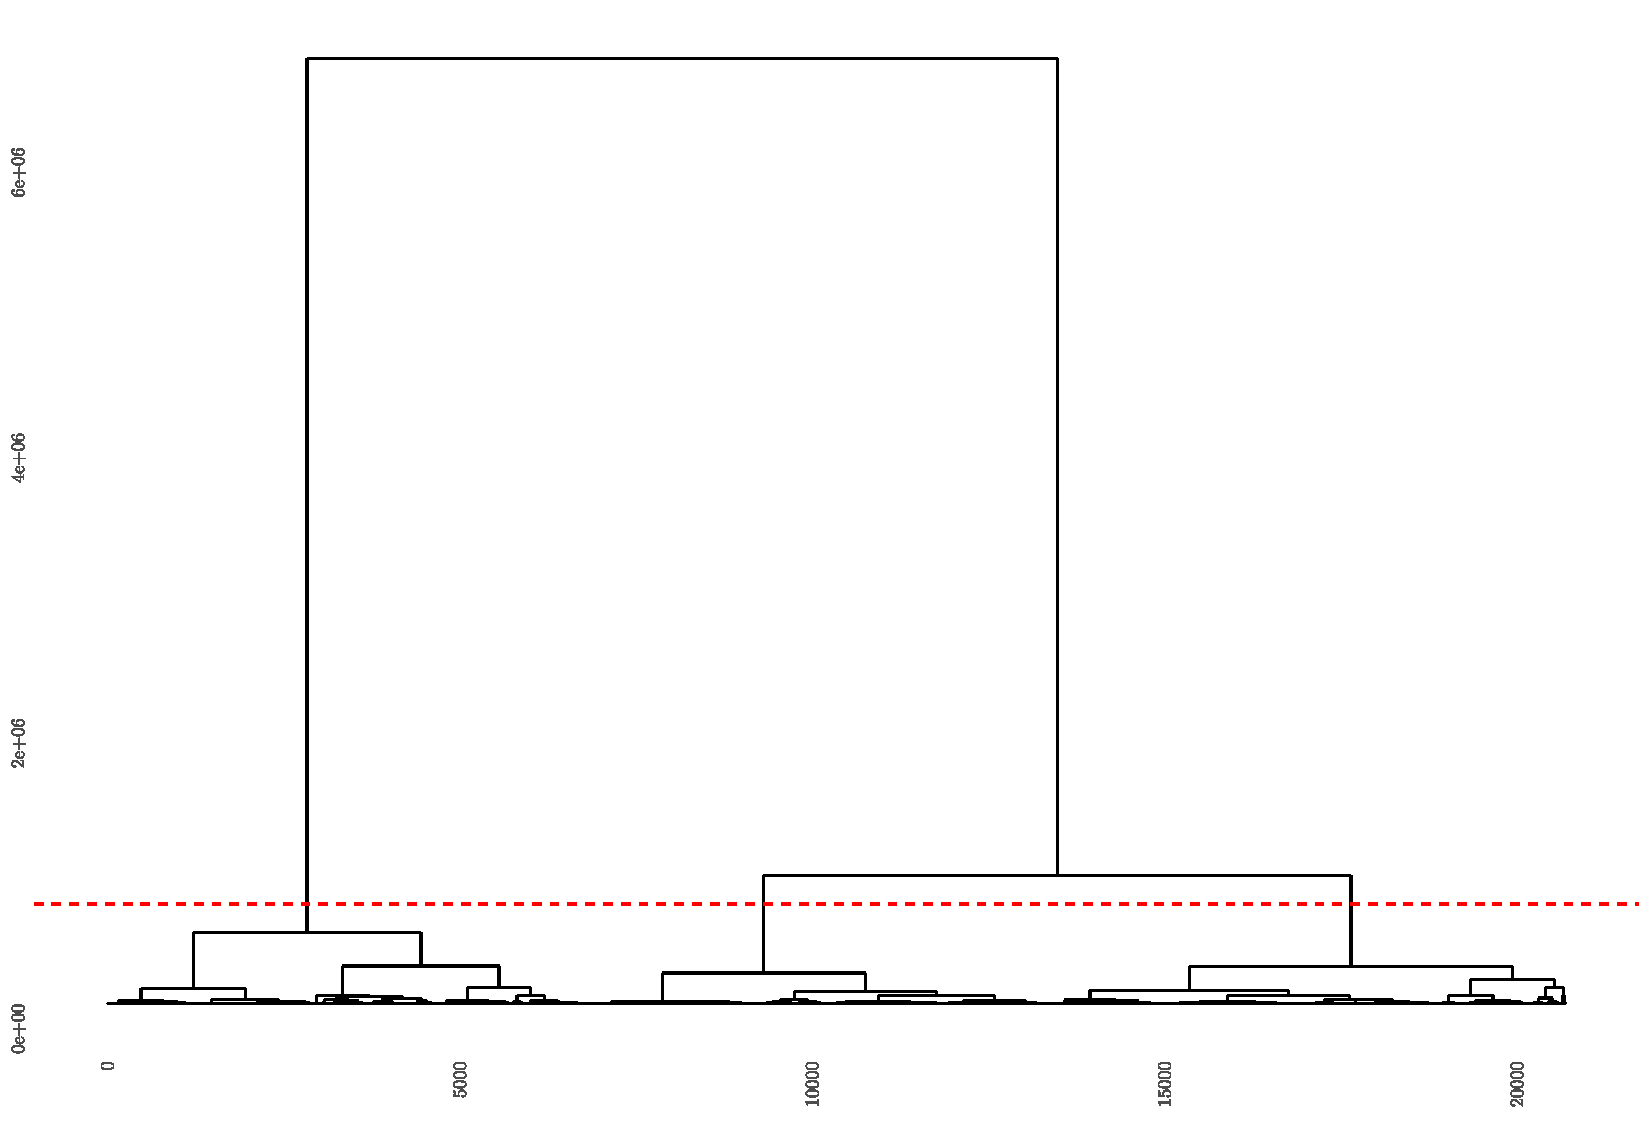
\includegraphics[width=0.8\linewidth]{dendo}
    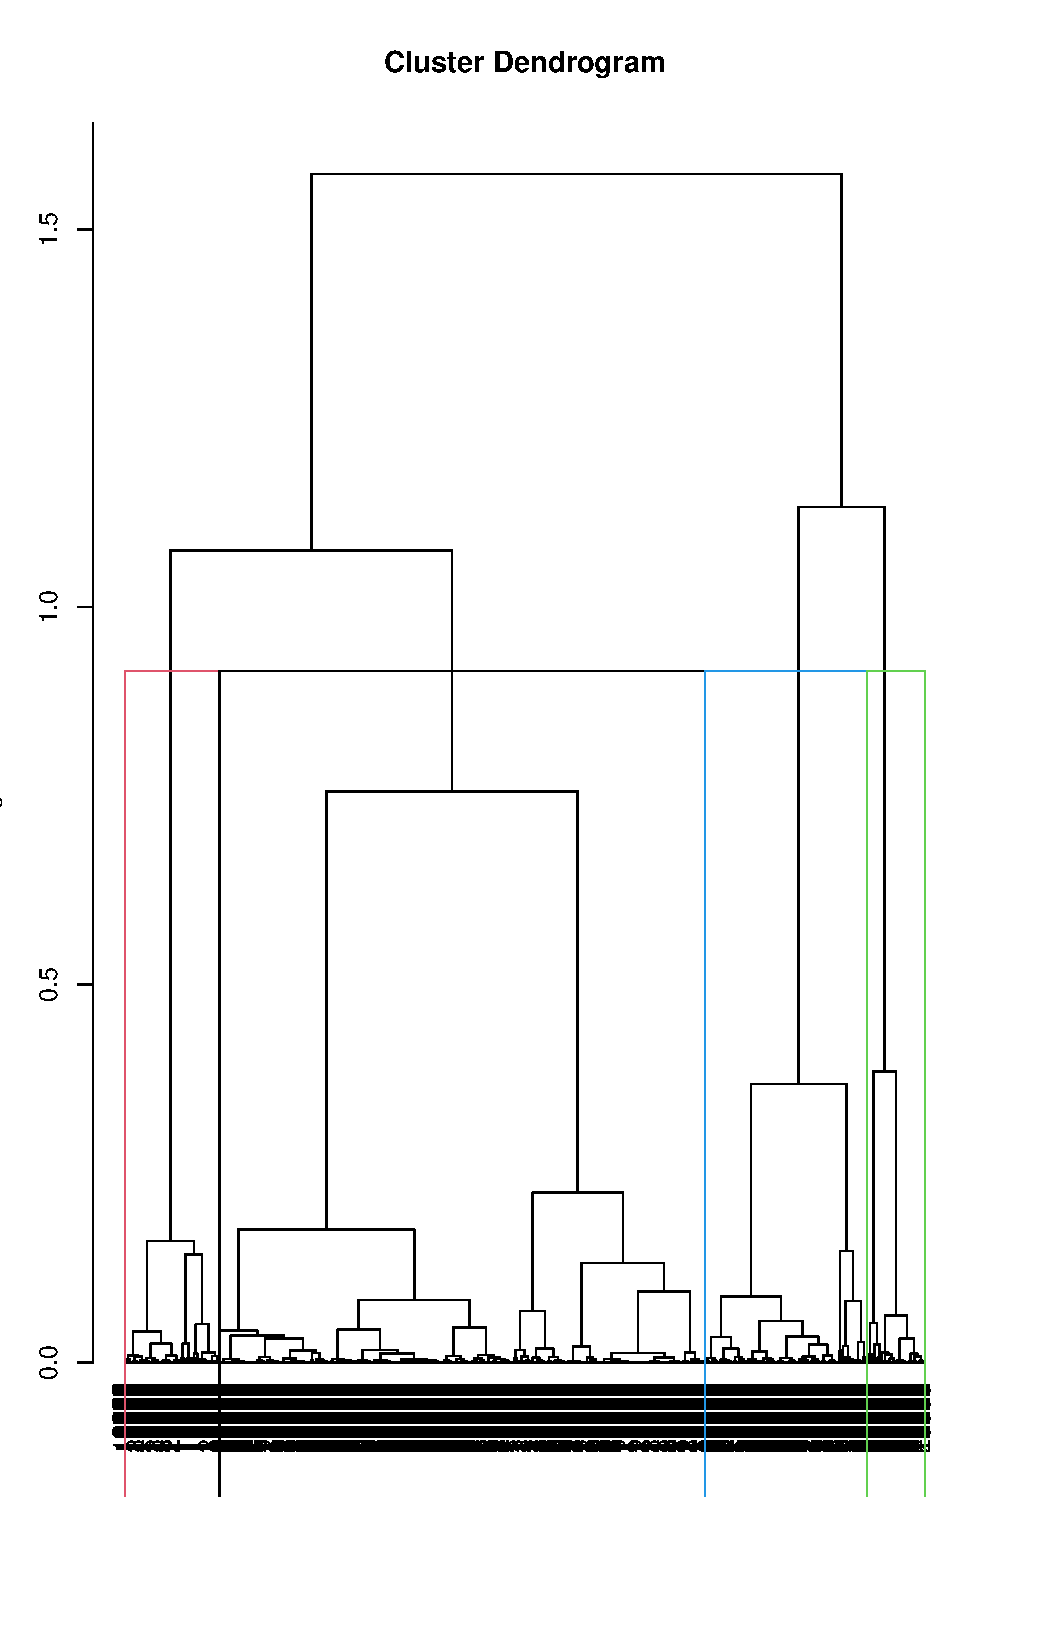
\includegraphics[width=0.8\linewidth]{cluster-dendo-h3}
    \caption{Cluster Dendogram}%
    \label{fig:dendogram}
\end{figure}

\end{landscape}


% Discuss about how to get the final number of clusters

\subsection{Description of clusters}%
\label{sub:description_of_clusters}

\begin{table}[H]
\centering
\caption{Cluster size table}%
\label{tab:cluster_size}

\begin{tabular}[t]{lr}
\toprule
c3 & Freq\\
\midrule
1 & 12733\\
2 & 2738\\
3 & 810\\
4 & 4414\\
\bottomrule
\end{tabular}
\end{table}


% Table with a description of the clusters size

%% vim: spell spelllang=en:
%! TEX root = **/00-main.tex

\section{Profiling of clusters}%
\label{sec:profiling_of_clusters}

\newcommand{\profiling}[3]{
\begin{figure}[H]
    \centering
    \includegraphics[width=0.7\textwidth]{prof-c3-#1-#2}
    \caption{#3}%
    \label{fig:prof-#1-#2}
\end{figure}
}

% --- cat

\profiling{host_is_superhost}{side}{Superhost distribution}
\profiling{host_since_year}{percent}{Host since year distribution}
In \Cref{fig:prof-host_is_superhost-side} we can see how cluster 2 has a significantly higher proportional amount of superhosts when comparing to the rest of cluster, while cluster 3 has very few of them. This could indicate that hosts in cluster 2 are better hosts, with more experience and a pretty good record of dealing with clients. The hypothesis is confirmed by \Cref{fig:prof-host_since_year-percent}, where, comparing the same two clusters we see a tendency: cluster 2 is composed mostly of veteran hosts whereas cluster 3 is made up of more novice ones.
%\profiling{host_is_superhost}{stack}{}


%\profiling{host_response_time}{}{} %?


\clearpage
\subsection{Room Types \& Accommdates}%

%profiling{room_type}{percent}{room type bar}
%\profiling{room_type}{stack}{room type bar}


% --- num

%\clearpage
%\subsection{Accommodates}%

%\profiling{accommodates}{vi}{Accommodates}
%\profiling{accommodates}{bp}{Accommodates}
\profiling{accommodates}{meanp}{Accommodates}
\profiling{room_type}{side}{room type bar}
In \Cref{fig:prof-accommodates-meanp} we can see that listings on cluster 4 accommodate
much more people than the ones in other clusters. By looking at \Cref{fig:prof-room_type-side}, we can correlate this with the fact that most of the listings on cluster 4 are entire houses or apartments, that usually accommodate more people than hotel rooms, private rooms or shared rooms. 

\clearpage
\subsection{Host listings count}%

\profiling{host_listings_count}{meanp}{Host listings count}
\profiling{host_listings_count}{bp}{Host listings count}
In \cref{fig:host_listings_count-meanp,fig:host_listings_count-bp} we can differences in the clusters.
Cluster 4 has the highest mean, followed by cluster 3. The other two seem to be quite 
similar. It might indicate that the hosts of the listings in cluster number 4 are actually businesses.

\profiling{price}{meanp-tallat200}{Price}
\profiling{price}{vi-tallat200}{Price}
When looking at \cref{fig:prof-price-meanp-tallat200,fig:prof-price-vi-tallat200} we can clearly see that the listings in cluster 4 have an average price way higher that the other ones. As we already found out that cluster 4 contains the listings that accommodate more guests as well. This makes sense because a house that can accommodate more guests is expected to be more expensive. 


\subsection{Review scores rating}%
\label{sub:prof-review_scores_rating}

\profiling{review_scores_rating}{meanp}{Review scores rating}
%\profiling{review_scores_rating}{vi}{Review scores rating}
\profiling{review_scores_rating}{bp}{Review scores rating}

Looking at \cref{fig:prof-review_scores_rating-meanp,fig:prof-review_scores_rating-bp} we can see that listings on cluster 3 have, on average, much lower review score rantings. The rest seem to have a really similar mean and variance. We can conclude that cluster 3 contains the bad reviews while high reviews seem to distribute between the others.

\clearpage
\subsection{Reviews per month}%

\profiling{reviews_per_month}{meanp}{Reviews per month}
%\profiling{reviews_per_month}{vi}{Reviews per month}
\profiling{reviews_per_month}{bp}{Reviews per month}

\Cref{fig:prof-reviews_per_month-bp,fig:prof-reviews_per_month-meanp} we can see that cluster 2 has higher mean that the rest and
cluster 3 has the lowest mean of them all.



% Profiling of clusters: Use class variable as a response variable to analyze
% conditional distributions of variables to clusters and eventual statistical
% tests to assess which variables are significant in each cluster. Detect
% commonalities of each cluster and differences between clusters. What is
% intrinsic of each cluster? What distinguishes clusters among them?

% Profiling graphs, CPGs, multiple boxplots, bivariate barplots, descriptive by
% groups, etc...

% For selected relevant variables, you can also add specific profiling tests to
% complete clusters interpretation

% Synthesize the result of the classes’ interpretation process into a set of
% templates characterizing the clusters, one template per cluster

%% vim: spell spelllang=en:
%! TEX root = **/00-main.tex

% Global discussion and general conclusions of the whole work. Analyze
% coincidences and divergences between ACP, AMC, Clustering

\section{Conclusions}%
\label{sec:conclusions}

One of the aims of the projects was to explain what variables have an effect on a customer leaving a good or bad review score. After doing the univariate analysis we found out that reviews were pretty polarized.  In fact, most of the scores were pretty high, but there was a small percentage of really bad ones. When analyzing the clusters created by HCPC, it turned out that we accumulated the really bad reviewed listings in cluster 3, while the other three contained mostly excellent scores. This made it hard for us to determine the characteristics of a good review. Because of that, we thought that it would be appropriate to study the characteristics of the listings that had bad review scores, since they were more distinguished and less broad. We concluded that most bad reviews tend to be posted on listings not owned by a superhost, that usually has a small number of preview reviews. We also found out that listings for shared rooms where more likely to end up having a bad review.

We also managed to conclude that cluster 4 contained mostly bigger and more expensive listings that could accommodate more guests. This is interesting but it doesn't help us answer any of the questions we had proposed at the beginning of the project.
In the opposite side of the spectrum,  cluster number 1 contains mostly the listings for the smaller apartments and private rooms, with good reviews and cheaper prices. This kind of listing seems to be the most popular one among Airbnb in Barcelona, which makes sense in our experience.

We have analysed further as to find any major difference between the clusters. Although some anecdotal facts have been found we don't think there's enough evidence to derive any further substantial differences.
%% vim: spell spelllang=en:
%! TEX root = **/00-main.tex

% Working plan, including (please be sure you include the working plan at the end
% of the document, not at the beginning)

% Initial and final Gantt

% vim: spell spelllang=en:
%! TEX root = **/00-main.tex

\begin{ganttchart}[
vgrid={*{6}{draw=none}, dotted},
x unit=.75cm,
y unit title=1cm,
y unit chart=1cm,
    time slot format=isodate
    %]{2020-09-15}{2020-10-07}
    ]{2020-09-15}{2020-10-28}
\gantttitlecalendar{month=name, day}
\ganttnewline

\ganttgroup{Motivation and Description}{2020-09-16}{2020-09-23}
\ganttnewline

\ganttgroup{Data source presentation}{2020-09-16}{2020-09-23}
\ganttnewline

\ganttbar{Description of data source}{2020-09-16}{2020-09-23}
\ganttnewline

\ganttgroup{Formal description of data structure}{2020-09-23}{2020-09-30}
\ganttnewline
\ganttbar{Metadata Table}{2020-09-23}{2020-09-25}
\ganttnewline
\ganttbar{Scope of study}{2020-09-25}{2020-09-30}
\ganttnewline

\ganttgroup{Description of preprocessing}{2020-09-23}{2020-09-27}
\ganttnewline

\ganttgroup{Basic statistical descriptive analysis}{2020-09-27}{2020-10-07}
\ganttnewline
\ganttbar{Univariate analysis}{2020-09-27}{2020-09-30}
\ganttnewline
\ganttbar{Bivariate analysis}{2020-10-01}{2020-10-04}
\ganttnewline
\ganttbar{Conclusion describing data}{2020-10-04}{2020-10-07}
\ganttnewline
%\end{ganttchart}
%
%\framebreak
%
%\begin{ganttchart}[
%vgrid={*{6}{draw=none}, dotted},
%x unit=.85cm,
%y unit title=1cm,
%y unit chart=1cm,
%    time slot format=isodate
%    ]{2020-10-07}{2020-10-28}
%\gantttitlecalendar{month=name, day}
%\ganttnewline

\ganttgroup{PCA analysis for numerical variables}{2020-10-07}{2020-10-14}
\ganttnewline
\ganttbar{Scree plot}{2020-10-07}{2020-10-11}
\ganttnewline
\ganttbar{Factorial map visualization}{2020-10-11}{2020-10-14}
\ganttnewline

\ganttgroup{Hierarchical Clustering}{2020-10-14}{2020-10-21}
\ganttnewline
\ganttbar{Clustering script}{2020-10-14}{2020-10-19}
\ganttnewline
\ganttbar{Description of data selected}{2020-10-19}{2020-10-21}
\ganttnewline
\ganttbar{Clustering method and metrics used}{2020-10-19}{2020-10-21}
\ganttnewline
\ganttbar{Resulting Dendogram}{2020-10-19}{2020-10-21}
\ganttnewline
\ganttbar{Discussion about number of clusters}{2020-10-19}{2020-10-21}
\ganttnewline
\ganttbar{Table with description of cluster size}{2020-10-19}{2020-10-21}
\ganttnewline

\ganttgroup{Profiling of clusters}{2020-10-21}{2020-10-28}
\ganttnewline
\ganttbar{Profiling graphs}{2020-10-21}{2020-10-28}
\ganttnewline

\end{ganttchart}

% vim: spell spelllang=en:
%! TEX root = **/00-main.tex

\newgeometry{top=0.5cm, bottom=0.5cm, left=0.5cm, right=0.5cm}
\begin{landscape}

\null
\vspace{1em}
{
\centering
\subsection{Final Gantt}%
\label{sub:fin_gantt}
\vspace{2em}
\par}

\begin{center}
\begin{ganttchart}[
vgrid={*{6}{draw=none}, dotted},
x unit=.75cm,
y unit title=1cm,
y unit chart=1cm,
    time slot format=isodate
    ]{2020-09-15}{2020-10-09}
\gantttitlecalendar{month=name, day}
\ganttnewline

\ganttgroup{Motivation and Description}{2020-09-16}{2020-09-21}
\ganttnewline

\ganttgroup{Data source presentation}{2020-09-16}{2020-09-22}
\ganttnewline

\ganttbar{Description of data source}{2020-09-16}{2020-09-22}
\ganttnewline

\ganttgroup{Formal description of data structure}{2020-09-23}{2020-09-30}
\ganttnewline
\ganttbar{Metadata Table}{2020-09-23}{2020-09-25}
\ganttnewline
\ganttbar{Scope of study}{2020-09-25}{2020-09-30}
\ganttnewline

\ganttgroup{Description of preprocessing}{2020-09-23}{2020-09-28}
\ganttnewline

\ganttgroup{Basic statistical descriptive analysis}{2020-09-27}{2020-10-09}
\ganttnewline
\ganttbar{Univariate analysis}{2020-09-27}{2020-09-02}
\ganttnewline
\ganttbar{Bivariate analysis}{2020-10-03}{2020-10-08}
\ganttnewline
\ganttbar{Conclusion describing data}{2020-10-08}{2020-10-09}
\ganttnewline
\end{ganttchart}
\end{center}

\pagebreak
\null
\vspace{3.5em}
\begin{center}
\begin{ganttchart}[
vgrid={*{6}{draw=none}, dotted},
x unit=.85cm,
y unit title=1cm,
y unit chart=1cm,
    time slot format=isodate
    ]{2020-10-07}{2020-10-28}
\gantttitlecalendar{month=name, day}
\ganttnewline

\ganttgroup{PCA analysis for numerical variables}{2020-10-07}{2020-10-12}
\ganttnewline
\ganttbar{Scree plot}{2020-10-07}{2020-10-10}
\ganttnewline
\ganttbar{Factorial map visualization}{2020-10-10}{2020-10-12}
\ganttnewline

\ganttgroup{Hierarchical Clustering}{2020-10-12}{2020-10-20}
\ganttnewline
\ganttbar{Clustering script}{2020-10-12}{2020-10-16}
\ganttnewline
\ganttbar{Description of data selected}{2020-10-17}{2020-10-18}
\ganttnewline
\ganttbar{Clustering method and metrics used}{2020-10-17}{2020-10-18}
\ganttnewline
\ganttbar{Resulting Dendogram}{2020-10-17}{2020-10-19}
\ganttnewline
\ganttbar{Discussion about number of clusters}{2020-10-19}{2020-10-20}
\ganttnewline
\ganttbar{Table with description of cluster size}{2020-10-19}{2020-10-20}
\ganttnewline

\ganttgroup{Profiling of clusters}{2020-10-20}{2020-10-26}
\ganttnewline
\ganttbar{Profiling graphs}{2020-10-20}{2020-10-26}
\ganttnewline

\end{ganttchart}
\end{center}
\end{landscape}

\restoregeometry
 

% Final tasks assignment grid

% vim: spell spelllang=en:
%! TEX root = **/00-main.tex

\subsection{Division of tasks}%
\label{sub:division_of_tasks}

\newcommand*\rot{\rotatebox{90}}
\newcommand*\X{\ding{56}}
\newcommand*\x{{\color{gray}\ding{55}}}
\begin{table}[H]
\centering
\begin{tabular}{@{}l|c|c|c|c@{}}
             & \rot{Aleix Boné} & \rot{Eduard Bosch} & \rot{David Gili} & \rot{Albert Mercadé} \\
\toprule
\textbf{Coordination}                           &    &    &\X  &    \\ \midrule
\textbf{Motivation and Description}             & \x &    &    & \X \\ \midrule
\textbf{Data source presentation}               &    &    &    &    \\
Description of data source                      &    & \x &    & \X \\ \midrule
\textbf{Formal description of data structure}   &    &    &    &    \\
Metadata Table                                  &\x  &\x  & \X &    \\
Scope of study                                  &\X  &\x  &    &    \\ \midrule
\textbf{Description of prepossessing}           &    &\X  &    & \x \\ \midrule
\textbf{Basic statistical descriptive analysis} &    &    &    &    \\
Univariate analysis                             &    &\x  &    & \X \\
Bivariate analysis                              &    & \x &\X  &    \\
Conclusion describing data                      &\X  & \x &    &    \\ \midrule
\textbf{PCA analysis for numerical variables}   &    &    &    &    \\
Scree plot                                      &    &    &\x  & \X \\
Factorial map visualization                     &    & \X & \x &    \\ \midrule
\textbf{Hierarchical Clustering}                &    &    &    &    \\
Clustering script                               &    & \X &    & \x \\
Description of data used                        &\x  &    & \X &    \\
Clustering method and metrics used              & \X &\x  &    &    \\
Resulting Dendogram                             &    &    &\X  &\x  \\
Discussion about number of clusters             &\x  &\X  &    &    \\
Table with description of cluster size          &\x  &    &\X  &    \\ \midrule
\textbf{Profiling of clusters}                  &    &    &    &    \\
Profiling graphs                                &    &    &\X  &\x  \\
\end{tabular}
\end{table}


\pagebreak
\subsection{Working plan conclusions}
As we can see, we didn't completely follow our plan in terms of timing, some stuff took more than we expected, and other things were easier than we thought, but in the end, we ended up finishing on time to review and prepare for the presentation.

Although we didn't have to make use of the contingency plan, our team was a 4-people team from the 2nd week of the project (because a member of our group changed subjects). This made us need to work harder than a the average 6-people team, but it also made it easier to work together, because there weren't as many opinions, which led to less noise whenever we had to take a decision. We didn't have many problems doing each data mining process, however our biggest challenge was making the final report and the presentation. In these tasks we would have loved to have an extra hand or two to comment some plots or enhance the presentation further.

% TODO
% Critical discussion about deviances of final scheduling with respect to the
% originally designed one and discussion about risks avoided by the initial
% contention plan and unexpected risks appeared during project.

%
%\printbibliography
%
%\appendix
%
%%% vim: spell spelllang=en:
%! TEX root = **/00-main.tex

% R Scripts (only if they have not been embedded along the explanations of the
% work in previous chapters)

\section{R Scripts}%
\label{sec:r_scripts}

% TODO explicacio de com va una mica...
The following subsections contain all the scripts used. There is a brief
explanation for each of them. They have to be run in the same working directory
with a \texttt{data} folder containing the data.

By default they produce and save all plots and tables to the file system
(although it will fail if there are no \texttt{plots/} and \texttt{tables/} in
the directory). To disable the PDF and table creation set the variables:
\mintinline{r}{savePlots <- FALSE; saveTables <- FALSE} before running the
scripts (see script in \cref{sub:shared.r} for details).

\newcommand{\mintedfile}[2]{
    \subsection{#1}%
    \label{sub:#1}
    #2
    \inputminted{r}{../../analysis/#1}
    \clearpage
}

%TODO add all files

\mintedfile{preprocessing.r}{
    Script used for the preprocessing data transformation explained in
    \cref{sec:preprocessing}
}
\mintedfile{descriptiveAnalysis.r}{
    Script used for univariate analysis (\cref{sub:univariate_analysis})
}
\mintedfile{NAtreatment.r}{
    Script used for \emph{NA} imputation.
}
\mintedfile{bivariate.r}{
    Script used for bivariate analysis (\cref{sub:bivariate_analysis})
}
\mintedfile{PCAcode.r}{
    Original script for PCA using built-in R methods. This was used in the exploration
    but in the end we decided to use the PCA with factorminer.
}
\mintedfile{zclusteringWithPC.r}{
    Script used for PCA with FactoMineR and clustering on this PCA.
}
\mintedfile{dendogram.r}{}
\mintedfile{profiling.r}{
    Script used for cluster profiling in \cref{sec:profiling_of_clusters}
}
\mintedfile{shared.r}{
    This script contains all shared code used to generate consistent plots and tables
    with \emph{ggplot2} and \emph{kable}.

    This script is sourced by all the other scripts that produce plots.

    To prevent it from generating pdf files set: \mintinline{r}{savePlots <- F}

    It has several dependencies used to generate tables and plots with latin
    modern font (\LaTeX{} font). If you don't want to use it or don't have it installed
    just set \mintinline{r}{fontsLoaded <- T} before sourcing the script.

}

%% vim: spell spelllang=en:
%! TEX root = **/00-main.tex

% Additional plots

\section{Additional plots}%
\label{sec:additional_plots}

\newcommand{\centroidmap}[2]{
    \begin{figure}[H]
        \centering
        \includegraphics[width=0.87\linewidth]{pca_fact-plane_#1_#2-cent}
        \caption{PCA plane #1 vs #2 (categorical variables centroids)}%
        \label{fig:plane_#1-#2-cent}
    \end{figure}
}

\begin{landscape}

\subsection{Categorical centroids on PCA planes}%
\label{sub:add_centroids}

\centroidmap{1}{2}
\centroidmap{1}{3}
\centroidmap{1}{4}
\centroidmap{2}{3}
\centroidmap{2}{4}
\centroidmap{3}{4}
\end{landscape}

% TODO

% es poden incluir a saco ajuntant els pdfs o amb un bucle o algo.
%\includepdf[pages=-,landscape=true]{../../analysis/plots/PCA_planes_sep}
%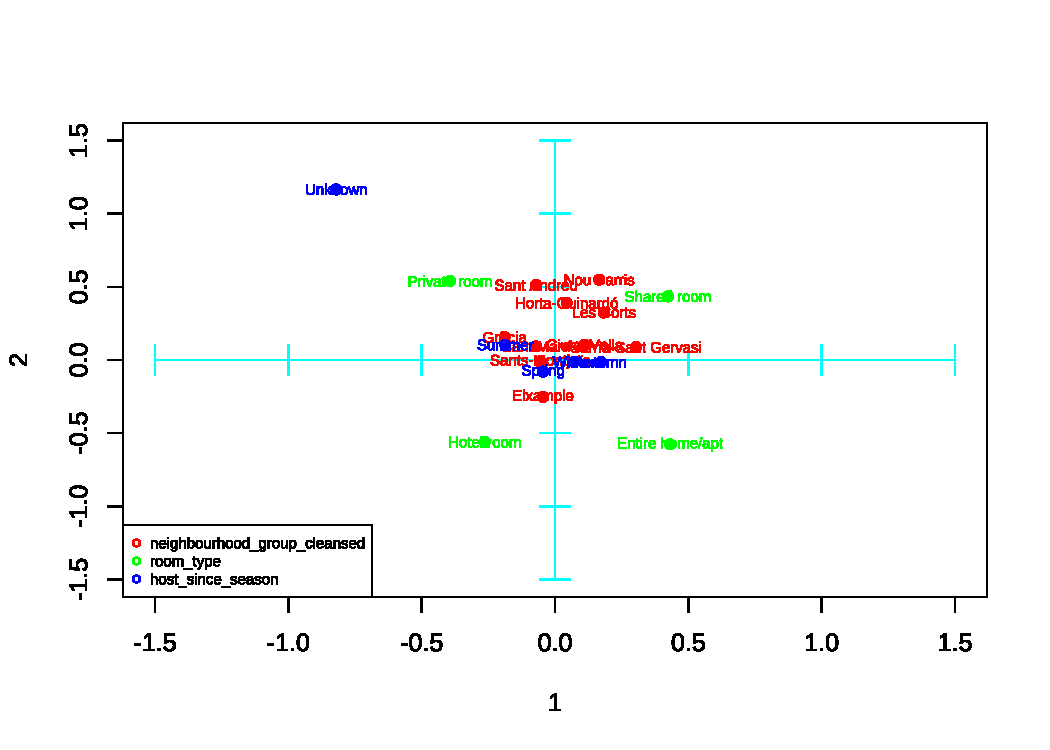
\includepdf[pages=-,landscape=true]{../../analysis/plots/PCA_planes_no_ordi}
%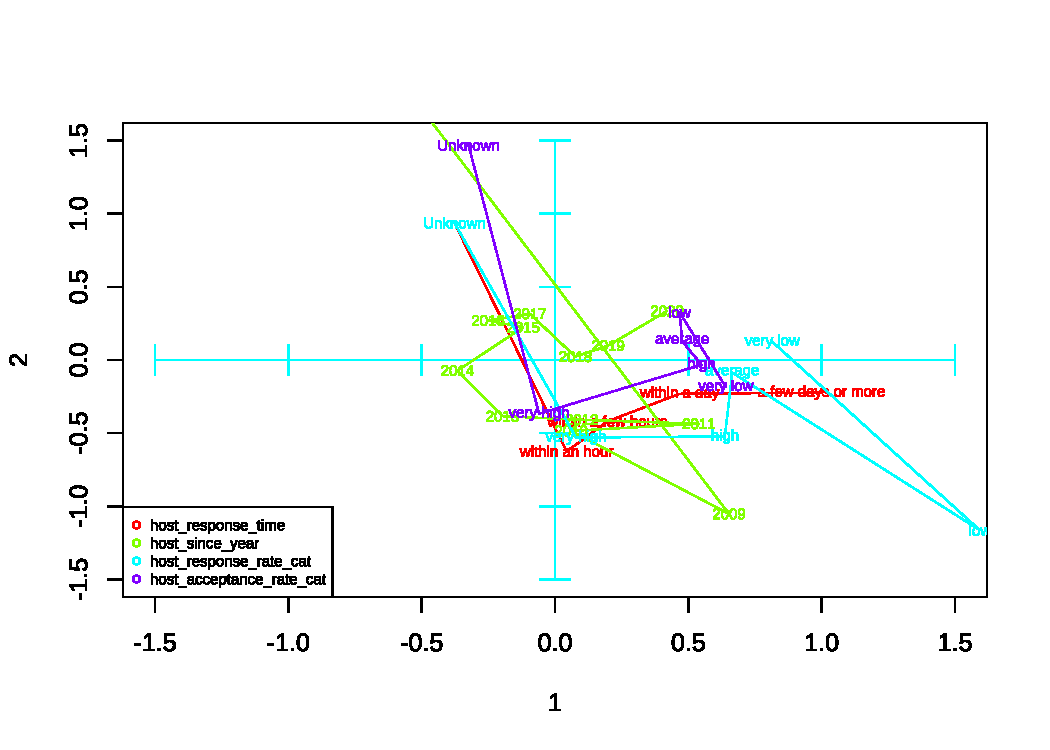
\includepdf[pages=-,landscape=true]{../../analysis/plots/PCA_planes_ordi}


\end{document}
